\documentclass[11pt,letterpaper,twoside]{book}

% ==========================================
% SIRCADA Reference Manual
% Picture processing unit, memory map and video modes
% ==========================================

% Manual-specific strings used by the shared preamble (footer, PDF metadata).
\newcommand{\sircManualFooter}{SIRCADA REFERENCE MANUAL}
\newcommand{\sircManualTitle}{SIRCADA Reference Manual}
\newcommand{\sircManualSubject}{SIRCADA, the SIRC Analogue Display Adapter: picture processing unit, memory map and video modes}

% Name of this manual, for references from the other manuals and within the set.
\newcommand{\videomanual}{\textit{SIRCADA Reference Manual}}

% ==========================================
% Shared preamble for the SIRC-1 manuals (docs/reference and docs/hardware)
% ==========================================

% ------------------------------------------------------------
% Encoding and typography
% ------------------------------------------------------------

\usepackage[utf8]{inputenc}
\usepackage[T1]{fontenc}

% Helvetica-compatible sans serif.
% TeX Gyre Heros is a high-quality Helvetica replacement.
\usepackage{tgheros}
\renewcommand{\familydefault}{\sfdefault}

% Courier-compatible monospace.
\usepackage{tgcursor}

% Better character spacing / kerning.
\usepackage{microtype}

% ------------------------------------------------------------
% Page layout
% ------------------------------------------------------------

\usepackage{geometry}

\geometry{
	a4paper,
	left=25mm,
	right=20mm,
	top=22mm,
	bottom=25mm,
	headheight=14pt
}

% The book class flushes page bottoms in two-sided mode. With many [H] tables
% that cuts pages short, so the leftover space gets spread through lists and
% paragraphs instead. Let short pages stay short.
\raggedbottom

% ------------------------------------------------------------
% General packages
% ------------------------------------------------------------

\usepackage{graphicx}
\usepackage{eso-pic}
\usepackage{xcolor}
\usepackage{fancyhdr}
\usepackage{titlesec}
\usepackage{enumitem}
\usepackage{float}

% A captioned, non-floating environment for worked assembly examples, so
% they get a real "List of Examples" (like the existing List of
% Figures/Tables) instead of a hand-maintained one. Numbered N-M (chapter
% number, then sequential within that chapter/appendix) to match the
% manual's existing "Example 13-1" convention; [H] means it never actually
% floats away from where the author placed it.
\newfloat{example}{H}{loe}[chapter]
\floatname{example}{Example}
\renewcommand{\theexample}{\thechapter-\arabic{example}}

\usepackage{tabularx}
\usepackage{booktabs}
\usepackage{multirow}
\usepackage{longtable}
\usepackage{xltabular}

\usepackage{amsmath}
\usepackage{amssymb}

\usepackage{listings}
\usepackage{bytefield}
\bytefieldsetup{endianness=big}

\usepackage{tikz}
\usepackage{tikz-timing}
\usetikzlibrary{
	shapes.geometric,
	arrows.meta,
	positioning,
	fit,
	calc
}

\usepackage{tcolorbox}
\tcbuselibrary{breakable, skins}

% Load hyperref relatively late.
\usepackage{hyperref}

% ------------------------------------------------------------
% Timing diagrams
% ------------------------------------------------------------

\tikzset{
	sirc timing diagram/.style={
			timing/slope=0,
			timing/dslope=0.15,
			timing/xunit=3.4em,
			timing/rowdist=2.2,
			timing/coldist=2.2,
		},
}

% ------------------------------------------------------------
% Colours
% ------------------------------------------------------------

\definecolor{sircred}{RGB}{255,0,0}
\definecolor{sircgray}{RGB}{110,110,110}
\definecolor{sirclightgray}{RGB}{232,232,232}
\definecolor{codebg}{RGB}{245,245,245}
\definecolor{opcodecolor}{RGB}{153,0,0}

% ------------------------------------------------------------
% Manual-specific strings
% ------------------------------------------------------------
% A manual's main.tex defines these (with \newcommand) before it inputs this
% preamble. The defaults are for the Architecture Reference Manual.

\providecommand{\sircManualFooter}{SIRC-1 ARCHITECTURE REFERENCE MANUAL}
\providecommand{\sircManualTitle}{SIRC-1 Architecture Reference Manual}
\providecommand{\sircManualSubject}{SIRCIS Instruction Set Architecture}

% Names of the manuals in the set, for references between them
\providecommand{\archmanual}{\textit{SIRC-1 Architecture Reference Manual}}
\providecommand{\hwmanual}{\textit{SIRC-1 Hardware Reference Manual}}
\providecommand{\asmmanual}{\textit{SIRC-1 Assembly Programmer's Manual}}

% ------------------------------------------------------------
% Header / footer
% ------------------------------------------------------------

\pagestyle{fancy}
\fancyhf{}

\fancyhead[LE]{\small\nouppercase{\leftmark}}
\fancyhead[RO]{\small\nouppercase{\rightmark}}
\fancyhead[RE,LO]{\small\textcolor{sircred}{DRAFT --- Not for Distribution}}

\fancyfoot[LE,RO]{\thepage}
\fancyfoot[C]{\small\textcolor{sircgray}{\sircManualFooter}}

\renewcommand{\headrulewidth}{0.8pt}
\renewcommand{\footrulewidth}{0.4pt}

% ------------------------------------------------------------
% PDF / hyperlink setup
% ------------------------------------------------------------

\hypersetup{
	colorlinks=true,
	linkcolor=sircred,
	filecolor=sircred,
	urlcolor=sircred,
	citecolor=sircred,
	bookmarksnumbered=true,
	pdfauthor={SIRC Development Team},
	pdftitle={\sircManualTitle},
	pdfsubject={\sircManualSubject},
}

% ------------------------------------------------------------
% Assembly code listings
% ------------------------------------------------------------

\lstdefinelanguage{SIRC}{
	morekeywords={
			ADDI,ADDR,ADCI,ADCR,SUBI,SUBR,SBCI,SBCR,
			ANDI,ANDR,ORRI,ORRR,XORI,XORR,
			LOAD,MOVI,MOVR,STOR,CMNI,CMNR,CNCI,CNCR,CMPI,CMPR,CPCI,CPCR,TSAI,TSAR,TSOI,TSOR,TSXI,TSXR,
			LDEA,LDEL,BRAN,LJMP,LJSR,BRSR,RETS,NOOP,
			WAIT,RETE,COPI,COPR,SHFT,EXCP,RSET,
			ETFR,ETTR,DMAR,DMAW,DMAT,MULU,MULS,DIVU,DIVS
		},
	keywordstyle=\color{sircred}\bfseries,
	sensitive=false,
	morecomment=[l]{;},
	commentstyle=\itshape\color{sircgray},
	morestring=[b]",
	stringstyle=\color{opcodecolor},
	basicstyle=\ttfamily\small,
	breaklines=true,
	showstringspaces=false
}

\lstset{
	language=SIRC,
	backgroundcolor=\color{codebg},
	frame=single,
	rulecolor=\color{sircgray},
	framesep=5pt,
	numbers=left,
	numberstyle=\tiny\color{sircgray},
	numbersep=7pt,
	xleftmargin=15pt,
	framexleftmargin=15pt,
	columns=fullflexible
}

% ------------------------------------------------------------
% Instruction reference pages
% ------------------------------------------------------------

% Modelled on the instruction-description pages of period CPU manuals (e.g.
% the M68000 Family Programmer's Reference Manual): each instruction gets a
% dedicated page (or run of pages) with the mnemonic set prominently at the
% top for flip-through lookup, rather than a boxed callout sitting in the
% middle of running text. \clearpage at the start of every entry guarantees
% two entries never share a page -- if one entry runs long, the next simply
% starts on the page after it ends. The chapter running header (already set
% by fancyhdr) carries the instruction category, matching how the M68000
% manual shows its category ("Integer Instructions", etc.) in the header of
% every instruction page.
%
% Every entry also gets its own table-of-contents/PDF-bookmark line, keyed
% off its own mnemonic and name, regardless of whether it sits directly
% under a \section of its own or is one of several instructions grouped
% under a shared \section (e.g. the Exception Unit meta-instructions in
% Chapter 16) -- so every instruction is individually findable via the ToC
% or bookmarks either way, matching the "flip through to find it" goal.
\newenvironment{instructionbox}[2]{%
	\clearpage
	\phantomsection
	\addcontentsline{toc}{section}{#1 -- #2}
	\noindent{\Huge\bfseries\color{sircred}#1}\par
	\vspace{3pt}
	\noindent{\Large\bfseries #2}\par
	\vspace{6pt}
	\titlerule
	\vspace{10pt}
}{%
}

% A compact boxed reference for one addressing mode: GENERATION, ASSEMBLER
% SYNTAX, FIELD ENCODING, and INSTRUCTION WORD COUNT, matching the M68000
% PRM's per-mode encoding box. Unlike instructionbox, this does not force a
% page break -- there are only seven addressing modes and each is short
% enough that several fit per page.
\newtcolorbox{addrmodebox}[1]{
	colback=sirclightgray,
	colframe=sircred,
	coltitle=black,
	fonttitle=\bfseries\large,
	title=#1,
	arc=0mm,
	boxrule=0.8pt,
	breakable,
	enhanced jigsaw,
}

% ------------------------------------------------------------
% Architectural notation
% ------------------------------------------------------------

\newcommand{\reg}[1]{\texttt{#1}}
\newcommand{\opcode}[1]{\textcolor{opcodecolor}{\texttt{0x#1}}}
\newcommand{\statusbit}[1]{\texttt{#1}}
\newcommand{\mnemonic}[1]{\textbf{\texttt{#1}}}
\newcommand{\addr}[1]{\texttt{#1}}
\newcommand{\imm}[1]{\texttt{\##1}}

\newcommand{\indirectimm}[2]{\texttt{(\##1, #2)}}
\newcommand{\indirectreg}[2]{\texttt{(#1, #2)}}
\newcommand{\postinc}[2]{\texttt{(#1, #2)+}}
\newcommand{\predec}[2]{\texttt{-(#1, #2)}}

\newcommand{\shift}[2]{\texttt{#1 \##2}}

% Active-low signal name with a period overbar, e.g. \activelow{BERR}
\newcommand{\activelow}[1]{\ensuremath{\overline{\mbox{#1}}}}

% ------------------------------------------------------------
% Chapter / section styling
% ------------------------------------------------------------

% Deliberately simple, mechanical headings rather than modern
% display typography.

\titleformat{\chapter}[display]
{\normalfont\bfseries\color{sircred}}
{\Large CHAPTER \thechapter}
{8pt}
{\Huge}
[\vspace{4pt}\titlerule]

\titlespacing*{\chapter}
{0pt}
{-10pt}
{28pt}

\titleformat{\section}
{\normalfont\Large\bfseries\color{sircred}}
{\thesection}
{1em}
{}

\titleformat{\subsection}
{\normalfont\large\bfseries\color{sircred}}
{\thesubsection}
{1em}
{}

\titleformat{\subsubsection}
{\normalfont\normalsize\bfseries}
{\thesubsubsection}
{1em}
{}

\titlespacing*{\section}
{0pt}
{2.5ex plus 0.5ex minus 0.2ex}
{1ex}

\titlespacing*{\subsection}
{0pt}
{2ex plus 0.5ex minus 0.2ex}
{0.8ex}

% ------------------------------------------------------------
% Tables
% ------------------------------------------------------------

\renewcommand{\arraystretch}{1.2}


\begin{document}

% Front Matter
\frontmatter
\AddToShipoutPictureBG*{%
	\put(0,0){
\includegraphics[width=\paperwidth,height=\paperheight]{../logos/cover-simple.jpg}}%
}

\begin{titlepage}
	\thispagestyle{empty}
	\centering

	\vspace*{2.5cm}

	
\includegraphics[width=0.45\textwidth]{../reference/sirc-logo.png}

	\vspace{0.8cm}

	{\Huge\bfseries\color{black} SIRCADA}

	\vspace{0.3cm}

	{\LARGE\bfseries\color{black} Reference Manual}

	\vspace{0.4cm}

	{\large\itshape\color{black} SIRC Analogue Display Adapter: Picture Processing Unit, Memory Map and Video Modes}

	\vfill

	{\small\color{black} SILICON INTEGRATED RESEARCH CORPORATION}

	\vspace{1cm}

\end{titlepage}

\chapter*{Preface}
\addcontentsline{toc}{chapter}{Preface}
\label{ch:preface}

\section*{About This Manual}

This manual documents SIRCADA, the SIRC Analogue Display Adapter: the picture processing unit (PPU) that turns tile,
tilemap and palette data in its own video memory into a 256 by 224 pixel picture. SIRCADA is a component in its own
right, in a package of its own. It is the companion to the \archmanual{}, which defines the SIRC-1 CPU, to the
\hwmanual{}, which defines the CPU package and bus, and to the \asmmanual{}, which defines the language used to program
them.

SIRCADA is a peripheral on a 16-bit bus, and any 16-bit processor that can supply a chip select, a bus strobe and a
read/write line can drive it. It was designed to work with the SIRC-1, so the signal names, the interrupt arrangements
and the programming examples in this manual are those of the SIRC-1.

It is written for:

\begin{itemize}
	\item Programmers writing graphics code for SIRCADA
	\item Authors of the tools that prepare tiles, tilemaps and palettes
	\item Engineers implementing the device, in hardware or in software
\end{itemize}

\section*{Assumed Knowledge}

This manual assumes familiarity with tile-based two-dimensional graphics hardware: tilemaps, palettes, scanline
rendering and the blanking intervals of a television signal. Readers who need the interrupt mechanism that delivers the
vertical sync signal to the CPU should read the exception chapters of the \archmanual{}.

\section*{Revision Status}

This is a working draft of the \videomanual{}, not for distribution. The device it describes is not finished.
Chapter~\ref{ch:status} lists, feature by feature, what has been built and what has not, and the questions still open;
it is a working record, and is not part of the specification of the device. Anything not yet decided elsewhere in the
manual is marked ``not yet specified''; the manual does not invent values for it.

\tableofcontents
\listoftables
\listoffigures

% Main Content
\mainmatter
\chapter{Introduction}
\label{ch:introduction}

\section{Purpose and Scope}

The SIRC-1 CPU is sold on its own, so it is documented in three manuals that stand apart from any system built around
it. SIRCADA is made for the SIRCUS system and has a manual of its own. Together the four manuals have the following
scopes:

\begin{table}[H]
	\centering
	\begin{tabular}{lp{8.2cm}}
		\toprule
		\textbf{Manual} & \textbf{Scope}                                                                                                          \\
		\midrule
		\archmanual{}   & ISA, instruction encodings, canonical assembly notation, exceptions, programmer-visible state                           \\
		\asmmanual{}    & Complete assembly syntax, directives, symbols, meta-instructions, and toolchain usage                                   \\
		\hwmanual{}     & Pinout, bus interface, timing, electrical characteristics                                                               \\
		\videomanual{}  & The picture processing unit: package and pinout, memory map, registers, data formats, video modes, timing (this manual) \\
		\bottomrule
	\end{tabular}
	\caption{The SIRC-1 and SIRCUS Manual Set}
	\label{tab:manual-set}
\end{table}

This manual covers SIRCADA as a component: its package and pins, what the CPU can read and write, how the device turns
the contents of its video memory into a picture, and the timing of its signals. It does not describe the CPU, its
instructions or its bus protocol. The device is a bus peripheral like any other, so the \hwmanual{} is authoritative
for how the CPU makes a bus cycle, and this manual is authoritative for how the device answers it and for what it does
once it has been reached.

\section{Device Overview}

The video device draws a picture one scanline at a time, with no frame buffer: for every group of four pixels it
fetches tilemap entries and tile data from its video memory, resolves them through a palette, and sends the result to
the display.

\begin{table}[H]
	\centering
	\begin{tabular}{lp{9cm}}
		\toprule
		\textbf{Property} & \textbf{Value}                                                                                                    \\
		\midrule
		Picture size      & 256 by 224 visible pixels (262 lines NTSC, 312 PAL; Chapter~\ref{ch:timing})                                      \\
		Colour            & 15 bits per pixel, 5 bits for each of red, green and blue                                                         \\
		Palette           & 256 entries of 16 bits, directly addressable by the CPU                                                           \\
		Video memory      & 32,768 words (64 KB), shared by tile data and tilemaps                                                            \\
		Tile data         & 4 bits per pixel                                                                                                  \\
		Backgrounds       & Four orthogonal in Mode 1; two isometric and one orthogonal in Mode 2; two orthogonal and one isometric in Mode 3 \\
		Sprites           & 128 entries, three layers, 32 per line (Chapter~\ref{ch:sprites})                                                 \\
		Interrupts        & Two: vertical sync (NMI) and line compare (IRQ4)                                                                  \\
		Line timing       & 1364 master clocks per line, 262 lines per frame                                                                  \\
		\bottomrule
	\end{tabular}
	\caption{Video Device Summary}
	\label{tab:device-summary}
\end{table}

\section{Video Modes}
\label{sec:video-modes}

The device has three video modes, selected by the \texttt{MODE} field of the Base Configuration register
(Section~\ref{sec:reg-base-config}). The modes share the memory map, the registers, the palette and the data formats.
They differ in how the backgrounds are drawn and in the fetch schedule that supports them.

\begin{table}[H]
	\centering
	\begin{tabular}{llp{7.5cm}}
		\toprule
		\textbf{Mode} & \textbf{\texttt{MODE} value} & \textbf{Description}                                                                                                 \\
		\midrule
		Mode 1        & 0                            & Four orthogonal backgrounds of square tiles and sprites. The reset mode.                                             \\
		Mode 2        & 1                            & Two isometric backgrounds: square tiles displayed as diamonds on a 2:1 ground plane, and an orthogonal status layer. \\
		Mode 3        & 2                            & One isometric background behind two orthogonal backgrounds.                                                          \\
		\bottomrule
	\end{tabular}
	\caption{Video Modes}
	\label{tab:video-modes}
\end{table}

Mode 1 is the conventional mode and is described in Chapter~\ref{ch:mode1}. Mode 2 is a specialised mode for games set
on a flat map seen from above at an angle. It is good at that and at little else; Chapter~\ref{ch:mode2} describes what
it does and, as importantly, what it gives up. Mode 3 (Chapter~\ref{ch:mode3}) keeps one isometric background and gives
the fetch slots of the other to two orthogonal ones. The values 3--7 of \texttt{MODE} are reserved; software must not
write them. The \texttt{MODE} field is sampled at the first cycle of each line, so a change takes effect at the start
of the next line.

\section{Block Diagrams}
\label{sec:block-diagrams}

Figure~\ref{fig:block-system} shows the device as the CPU sees it: four areas of memory behind one bus interface, a
video output, and two interrupt lines. Figure~\ref{fig:block-ppu} shows what is inside. The chapters that follow
describe each block; the figure says how they feed each other.

\begin{figure}[H]
	\centering
	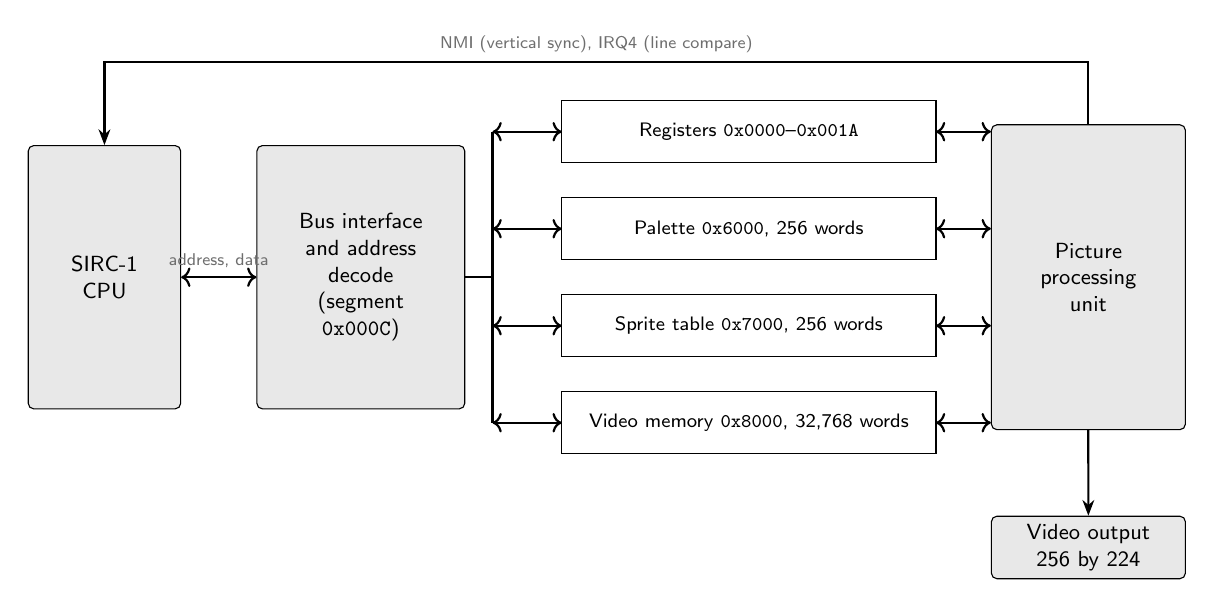
\begin{tikzpicture}[
			scale=0.88, transform shape,
			block/.style={draw, rounded corners=2pt, fill=sirclightgray, align=center, font=\small},
			mem/.style={draw, fill=white, align=center, font=\footnotesize, minimum height=0.9cm, minimum width=5.4cm},
			flow/.style={-{Stealth[length=2mm]}, thick},
			note/.style={font=\scriptsize, text=sircgray}
		]
		\node[block, minimum width=2.2cm, minimum height=3.8cm] (cpu) at (0,0) {SIRC-1\\CPU};
		\node[block, minimum width=3.0cm, minimum height=3.8cm] (bus) at (3.7,0) {Bus interface\\and address\\decode\\(segment\\\texttt{0x000C})};
		\node[mem] (m1) at (9.3,2.1) {Registers \texttt{0x0000}--\texttt{0x001A}};
		\node[mem] (m2) at (9.3,0.7) {Palette \texttt{0x6000}, 256 words};
		\node[mem] (m3) at (9.3,-0.7) {Sprite table \texttt{0x7000}, 256 words};
		\node[mem] (m4) at (9.3,-2.1) {Video memory \texttt{0x8000}, 32,768 words};
		\node[block, minimum width=2.8cm, minimum height=4.4cm] (ppu) at (14.2,0) {Picture\\processing\\unit};
		\node[block, minimum width=2.8cm] (out) at (14.2,-3.9) {Video output\\256 by 224};
		\draw[flow, <->] (cpu) -- node[above, note]{address, data} (bus);
		\draw[thick] (5.6,2.1) -- (5.6,-2.1);
		\draw[thick] (bus.east) -- (5.6,0);
		\foreach \y in {2.1,0.7,-0.7,-2.1} {
				\draw[flow, <->] (5.6,\y) -- (6.6,\y);
				\draw[flow, <->] (12.0,\y) -- (ppu.west |- 0,\y);
			}
		\draw[flow] (ppu) -- (out);
		\draw[flow] (ppu.north) -- ++(0,0.9) -| node[above, near start, note]{NMI (vertical sync), IRQ4 (line compare)} (cpu.north);
	\end{tikzpicture}
	\caption{The Video Device in the System}
	\label{fig:block-system}
\end{figure}

\begin{figure}[H]
	\centering
	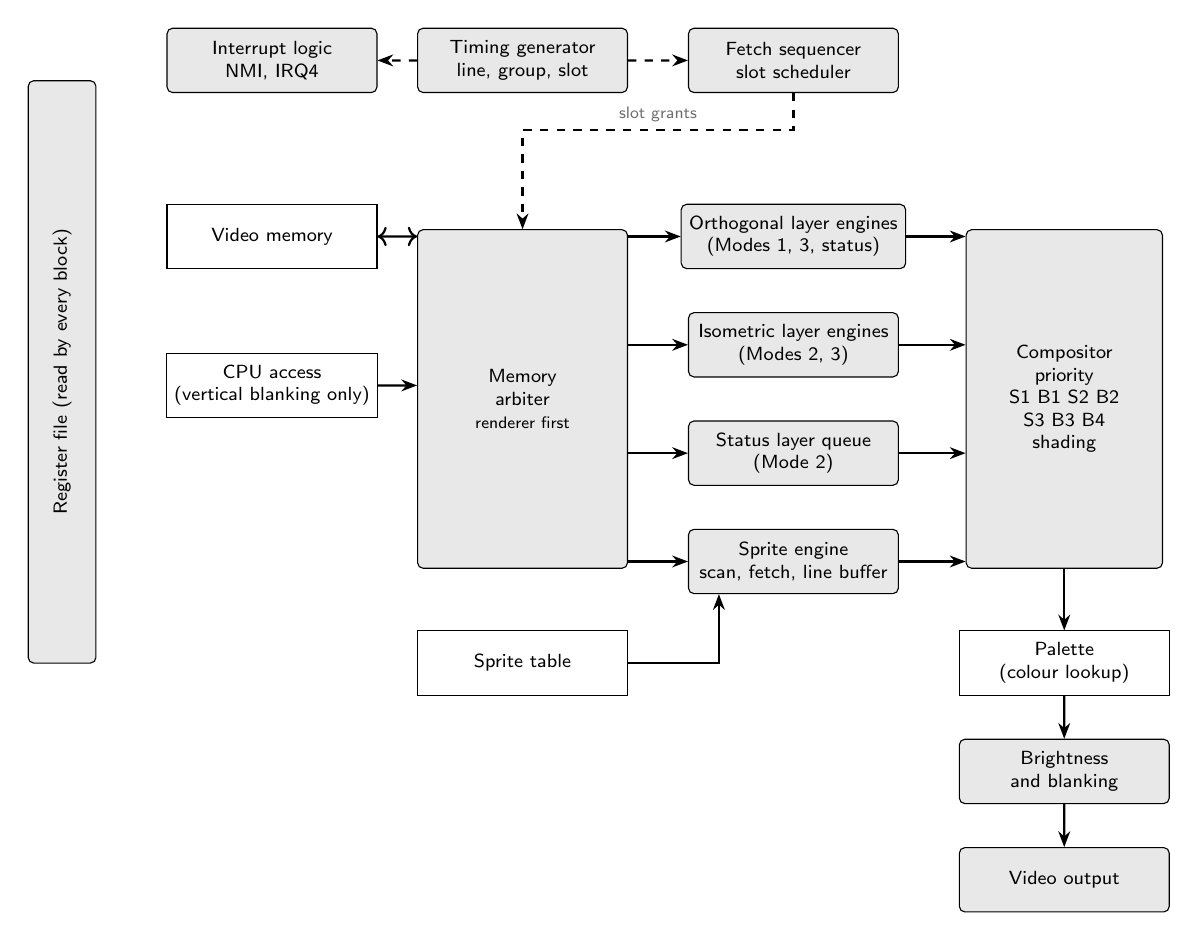
\begin{tikzpicture}[
			scale=0.86, transform shape,
			block/.style={draw, rounded corners=2pt, fill=sirclightgray, align=center, font=\footnotesize, minimum height=0.95cm, minimum width=3.1cm},
			store/.style={draw, fill=white, align=center, font=\footnotesize, minimum height=0.95cm, minimum width=3.1cm},
			flow/.style={-{Stealth[length=2mm]}, thick},
			ctl/.style={-{Stealth[length=2mm]}, thick, dashed},
			note/.style={font=\scriptsize, text=sircgray}
		]
		% Register file runs down the left edge: every block reads it
		\node[block, minimum width=8.6cm, minimum height=1.0cm, rotate=90] (regs) at (-1.5,3.4) {Register file (read by every block)};
		% Control row
		\node[block] (intr) at (1.6,8.0) {Interrupt logic\\NMI, IRQ4};
		\node[block] (timing) at (5.3,8.0) {Timing generator\\line, group, slot};
		\node[block] (seq) at (9.3,8.0) {Fetch sequencer\\slot scheduler};
		% Column 1: memories and CPU
		\node[store] (vram) at (1.6,5.4) {Video memory};
		\node[store] (cpu) at (1.6,3.2) {CPU access\\(vertical blanking only)};
		\node[store] (oam) at (5.3,-0.9) {Sprite table};
		% Column 2: arbiter
		\node[block, minimum height=5.0cm] (arb) at (5.3,3.0) {Memory\\arbiter\\\scriptsize renderer first};
		% Column 3: engines
		\node[block] (flat) at (9.3,5.4) {Orthogonal layer engines\\(Modes 1, 3, status)};
		\node[block] (iso) at (9.3,3.8) {Isometric layer engines\\(Modes 2, 3)};
		\node[block] (que) at (9.3,2.2) {Status layer queue\\(Mode 2)};
		\node[block] (spe) at (9.3,0.6) {Sprite engine\\scan, fetch, line buffer};
		% Column 4: compositor and output
		\node[block, minimum height=5.0cm, minimum width=2.9cm] (comp) at (13.3,3.0) {Compositor\\priority\\S1 B1 S2 B2\\S3 B3 B4\\shading};
		\node[store] (pal) at (13.3,-0.9) {Palette\\(colour lookup)};
		\node[block] (bri) at (13.3,-2.5) {Brightness\\and blanking};
		\node[block] (vo) at (13.3,-4.1) {Video output};
		% Control flows
		\draw[ctl] (timing) -- (intr);
		\draw[ctl] (timing) -- (seq);
		\draw[ctl] (seq.south) -- ++(0,-0.55) -| node[above, near start, note]{slot grants} (arb.north);
		% Data flows
		\draw[flow, <->] (vram) -- (vram.east -| arb.west);
		\draw[flow] (cpu) -- (cpu.east -| arb.west);
		\draw[flow] (oam.east) -| ([xshift=-1.1cm]spe.south);
		\foreach \e in {flat,iso,que} { \draw[flow] (arb.east |- \e) -- (\e.west); }
		\draw[flow] (arb.east |- spe) -- (spe.west);
		\foreach \e in {flat,iso,que,spe} { \draw[flow] (\e.east) -- (\e.east -| comp.west); }
		\draw[flow] (comp.south) -- (pal.north);
		\draw[flow] (pal) -- (bri);
		\draw[flow] (bri) -- (vo);
	\end{tikzpicture}
	\caption{Blocks of the Picture Processing Unit}
	\label{fig:block-ppu}
\end{figure}

\section{Conventions}

\begin{itemize}
	\item All addresses and sizes are in 16-bit words, as on the CPU. A word address is an offset from the base of the device's
	      segment unless stated otherwise.
	\item Bit 0 is the least significant bit. Bit diagrams draw the most significant bit on the left.
	\item Hexadecimal values carry a \texttt{0x} prefix and upper case digits.
	\item Ranges of values and addresses use an en dash: \texttt{0x0000}--\texttt{0x00FF}.
	\item \textbf{Reserved} fields and registers are set aside by the architecture. Software must not rely on what they
	      read, and should write zero to a reserved field it does not otherwise use.
	\item A value that the design has not fixed is \textbf{not yet specified}. It is not undefined, and no value is implied.
\end{itemize}

\chapter{Package and Pinout}
\label{ch:package}

The video device is a single integrated circuit with its video memory in separate static RAM chips. The picture
processing unit, the palette, the sprite table and the colour converters are on the one piece of silicon. The 64 KB of
video memory is outside it, on a memory bus of its own, so besides the bus of the CPU, two interrupt outputs, the clock
and reset inputs and the video output, the package carries the signals of that memory bus. This chapter gives the
package, the meaning of every pin and the timing the video memory must meet. Chapter~\ref{ch:signal-timing} gives the
timing of the signals.

\section{Chip Layout}

The device is supplied in a 100-pin plastic quad flat package (QFP-100), 25 pins on each side. Pin 1 is at the top left
corner, marked by a dot on the package; the pins are numbered counter-clockwise when the package is seen from above.

\begin{figure}[H]
	\centering
	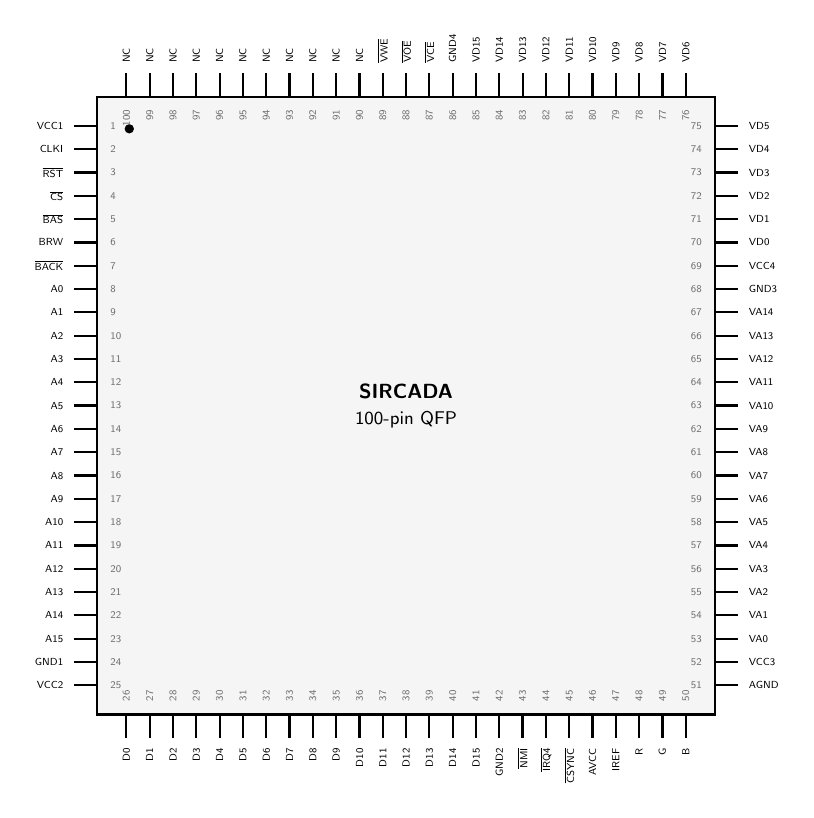
\begin{tikzpicture}[
			scale=0.74, transform shape,
			pinlabel/.style={font=\tiny},
			pinnum/.style={font=\tiny, text=sircgray},
			body/.style={draw, thick, fill=gray!8},
			pin/.style={draw, thick}
		]
		\def\pitch{0.4}
		\def\side{10.6}
		\def\first{0.5}
		% Package body
		\draw[body] (0,0) rectangle (\side,\side);
		% Pin 1 index dot
		\fill (0.55,\side-0.55) circle (0.08);
		% Left side, top to bottom: pins 1 to 25
		\foreach \n/\name [count=\i from 0] in {
				1/VCC1, 2/CLKI, 3/\activelow{RST}, 4/\activelow{CS}, 5/\activelow{BAS}, 6/BRW, 7/\activelow{BACK}, 8/A0,
				9/A1, 10/A2, 11/A3, 12/A4, 13/A5, 14/A6, 15/A7, 16/A8,
				17/A9, 18/A10, 19/A11, 20/A12, 21/A13, 22/A14, 23/A15, 24/GND1,
				25/VCC2
			} {
				\pgfmathsetmacro{\y}{\side - \first - \i*\pitch}
				\draw[pin] (0,\y) -- (-0.4,\y);
				\node[pinnum, anchor=west] at (0.1,\y) {\n};
				\node[pinlabel, anchor=east] at (-0.46,\y) {\name};
			}
		% Bottom side, left to right: pins 26 to 50
		\foreach \n/\name [count=\i from 0] in {
				26/D0, 27/D1, 28/D2, 29/D3, 30/D4, 31/D5, 32/D6, 33/D7,
				34/D8, 35/D9, 36/D10, 37/D11, 38/D12, 39/D13, 40/D14, 41/D15,
				42/GND2, 43/\activelow{NMI}, 44/\activelow{IRQ4}, 45/\activelow{CSYNC}, 46/AVCC, 47/IREF, 48/R, 49/G,
				50/B
			} {
				\pgfmathsetmacro{\x}{\first + \i*\pitch}
				\draw[pin] (\x,0) -- (\x,-0.4);
				\node[pinnum, rotate=90, anchor=west] at (\x,0.1) {\n};
				\node[pinlabel, rotate=90, anchor=east] at (\x,-0.46) {\name};
			}
		% Right side, bottom to top: pins 51 to 75
		\foreach \n/\name [count=\i from 0] in {
				51/AGND, 52/VCC3, 53/VA0, 54/VA1, 55/VA2, 56/VA3, 57/VA4, 58/VA5,
				59/VA6, 60/VA7, 61/VA8, 62/VA9, 63/VA10, 64/VA11, 65/VA12, 66/VA13,
				67/VA14, 68/GND3, 69/VCC4, 70/VD0, 71/VD1, 72/VD2, 73/VD3, 74/VD4,
				75/VD5
			} {
				\pgfmathsetmacro{\y}{\first + \i*\pitch}
				\draw[pin] (\side,\y) -- (\side+0.4,\y);
				\node[pinnum, anchor=east] at (\side-0.1,\y) {\n};
				\node[pinlabel, anchor=west] at (\side+0.46,\y) {\name};
			}
		% Top side, right to left: pins 76 to 100
		\foreach \n/\name [count=\i from 0] in {
				76/VD6, 77/VD7, 78/VD8, 79/VD9, 80/VD10, 81/VD11, 82/VD12, 83/VD13,
				84/VD14, 85/VD15, 86/GND4, 87/\activelow{VCE}, 88/\activelow{VOE}, 89/\activelow{VWE}, 90/NC, 91/NC,
				92/NC, 93/NC, 94/NC, 95/NC, 96/NC, 97/NC, 98/NC, 99/NC,
				100/NC
			} {
				\pgfmathsetmacro{\x}{\side - \first - \i*\pitch}
				\draw[pin] (\x,\side) -- (\x,\side+0.4);
				\node[pinnum, rotate=90, anchor=east] at (\x,\side-0.1) {\n};
				\node[pinlabel, rotate=90, anchor=west] at (\x,\side+0.46) {\name};
			}
		% Package label
		\node[font=\bfseries] at (\side/2,\side/2+0.25) {SIRCADA};
		\node[font=\small] at (\side/2,\side/2-0.25) {100-pin QFP};
	\end{tikzpicture}
	\caption{SIRCADA 100-pin QFP Pinout, Top View}
	\label{fig:pinout}
\end{figure}

\begin{table}[H]
	\centering
	\begin{tabular}{rll}
		\toprule
		\textbf{Pin} & \textbf{Name}     & \textbf{Description}              \\
		\midrule
		1            & VCC1              & Power supply                      \\
		2            & CLKI              & Clock input                       \\
		3            & \activelow{RST}   & Reset input                       \\
		4            & \activelow{CS}    & Chip select input                 \\
		5            & \activelow{BAS}   & Bus access strobe input           \\
		6            & BRW               & Bus read/write input              \\
		7            & \activelow{BACK}  & Bus acknowledge output            \\
		8--23        & A0--A15           & Address bus bits 0--15            \\
		24           & GND1              & Ground                            \\
		25           & VCC2              & Power supply                      \\
		26--41       & D0--D15           & Data bus bits 0--15               \\
		42           & GND2              & Ground                            \\
		43           & \activelow{NMI}   & Vertical sync interrupt output    \\
		44           & \activelow{IRQ4}  & Line-compare interrupt output     \\
		45           & \activelow{CSYNC} & Composite sync output             \\
		46           & AVCC              & Analog power supply               \\
		47           & IREF              & Colour output reference           \\
		48--50       & R, G, B           & Analog colour outputs             \\
		51           & AGND              & Analog ground                     \\
		52           & VCC3              & Power supply                      \\
		53--67       & VA0--VA14         & Video memory address bits 0--14   \\
		68           & GND3              & Ground                            \\
		69           & VCC4              & Power supply                      \\
		70--85       & VD0--VD15         & Video memory data bits 0--15      \\
		86           & GND4              & Ground                            \\
		87           & \activelow{VCE}   & Video memory chip enable output   \\
		88           & \activelow{VOE}   & Video memory output enable output \\
		89           & \activelow{VWE}   & Video memory write enable output  \\
		90--100      & NC                & No connection                     \\
		\bottomrule
	\end{tabular}
	\caption{SIRCADA 100-pin QFP Pinout}
	\label{tab:pinout}
\end{table}

\section{Signal Descriptions}

Table~\ref{tab:signals} lists the direction and sense of each signal. Active-low signals carry a bar over the name;
they are asserted when low. Address and data signals are active high. An output marked \emph{open drain} can only pull
its line low; the system supplies a pull-up, and several devices may share the line.

\begin{table}[H]
	\centering
	\small
	\begin{tabularx}{\textwidth}{llllX}
		\toprule
		\textbf{Signal}   & \textbf{Pins} & \textbf{Direction} & \textbf{Output type} & \textbf{Function}                             \\
		\midrule
		CLKI              & 2             & Input              &                      & Rising edge advances the device one PPU cycle \\
		\activelow{RST}   & 3             & Input              &                      & Resets the device                             \\
		\activelow{CS}    & 4             & Input              &                      & Selects the device for a bus cycle            \\
		\activelow{BAS}   & 5             & Input              &                      & Marks a bus cycle                             \\
		BRW               & 6             & Input              &                      & High for a read, low for a write              \\
		\activelow{BACK}  & 7             & Output             & Open drain           & Completes the bus cycle                       \\
		A0--A15           & 8--23         & Input              &                      & Word offset in the device segment             \\
		D0--D15           & 26--41        & Bidirectional      & Three-state          & Data                                          \\
		\activelow{NMI}   & 43            & Output             & Open drain           & Vertical sync interrupt                       \\
		VA0--VA14         & 53--67        & Output             & Driven               & Video memory word address                     \\
		VD0--VD15         & 70--85        & Bidirectional      & Three-state          & Video memory data                             \\
		\activelow{VCE}   & 87            & Output             & Driven               & Enables the video memory                      \\
		\activelow{VOE}   & 88            & Output             & Driven               & Video memory drives its data                  \\
		\activelow{VWE}   & 89            & Output             & Driven               & Video memory takes a word                     \\
		\activelow{IRQ4}  & 44            & Output             & Open drain           & Line-compare interrupt                        \\
		\activelow{CSYNC} & 45            & Output             & Driven               & Composite sync                                \\
		R, G, B           & 48--50        & Output             & Analog               & Colour                                        \\
		IREF              & 47            & Reference          &                      & Sets the full-scale colour level              \\
		\bottomrule
	\end{tabularx}
	\caption{Signal Summary}
	\label{tab:signals}
\end{table}

\subsection{Clock Input (CLKI)}

The device has one clock input, the same \texttt{CLKI} the system supplies to the CPU. One \texttt{CLKI} cycle is one
PPU cycle: the master clock divided by two (Section~\ref{sec:cpu-clock}). Every internal interval, the pixel, the group
of four pixels, the line and the frame, is a whole number of \texttt{CLKI} cycles, so the device needs no other clock.
The pixel rate is \texttt{CLKI} divided by two. The rising edge is the only edge the device uses. The range of clock
frequencies is not yet specified.

\subsection{Reset Input (\activelow{RST})}

While \activelow{RST} is asserted the device is held in its reset state (Section~\ref{sec:signal-reset}). The input is
sampled on each rising edge of \texttt{CLKI}, and must stay asserted for at least six cycles. The \activelow{RSTO}
output of the CPU holds for at least that long and can be connected directly.

\subsection{Bus Signals}

The device is a bus peripheral. It watches the bus of the CPU (\hwmanual{}) and answers the cycles that are addressed
to it. It has no byte strobes and no access-type inputs: it treats an instruction fetch, a data access and a DMA
transfer alike.

\begin{description}
	\item[\activelow{CS}] The system decodes the segment of the device, the upper address bits that the device does not see, and
	      asserts \activelow{CS} while the segment is addressed. A cycle in which \activelow{CS} or \activelow{BAS} is
	      deasserted is ignored: the device drives neither the data bus nor \activelow{BACK}.
	\item[\activelow{BAS}, BRW] The CPU asserts \activelow{BAS} for a whole cycle that makes a bus access. BRW is high for a
	      read and low for a write. Both are valid for the whole of the cycle.
	\item[A0--A15] The word offset of the access within the segment (Chapter~\ref{ch:memory-map}). The device accesses one 16-bit
	      word per cycle.
	\item[D0--D15] On a write the CPU drives the bus and the device takes the word at the rising edge that ends the cycle. On a
	      read the device drives the word that the offset selects, from the start of the cycle to its end, and releases the bus
	      when the cycle ends. A read of an offset that has no register or memory is driven as zero.
	\item[\activelow{BACK}] The device asserts \activelow{BACK} for the whole of every cycle in which \activelow{CS} and \activelow{BAS} are asserted, whatever the offset and whatever the state of the picture, with one exception: for a read of video memory it holds \activelow{BACK} off for the first cycle, which makes the CPU wait one cycle (Section~\ref{sec:signal-vram}), or two when a write to video memory immediately precedes it. It never raises a bus error. \activelow{BACK} is open drain, so it may be joined with the acknowledge from other devices on the bus.
\end{description}

\subsection{Video Memory Bus (VA0--VA14, VD0--VD15, \activelow{VCE}, \activelow{VOE}, \activelow{VWE})}
\label{sec:package-vram-bus}

The video memory is 32,768 words of 16 bits, for instance two static RAMs of 32,768 by 8 bits, one for the low byte and
one for the high byte of every word. The device is the only master of this bus. The CPU reaches video memory through
the device, in the cycles the renderer leaves free (Section~\ref{sec:memory-vram-access}).

\begin{description}
	\item[VA0--VA14] The word address of the access. Address bit 15 of the offset in the segment (\texttt{0x8000}) selects video
	      memory and is not part of this address.
	\item[VD0--VD15] On a read the memory drives the word and the device takes it at the rising edge of \texttt{CLKI} that ends
	      the cycle. On a write the device drives the word for the whole of the cycle in which \activelow{VWE} is asserted.
	\item[\activelow{VCE}, \activelow{VOE}, \activelow{VWE}] \activelow{VCE} is asserted in every cycle in which the device
	      accesses the memory. \activelow{VOE} is asserted as well for a read and \activelow{VWE} for a write.
\end{description}

The memory must meet the requirements of Table~\ref{tab:vram-timing}, which are those of one access in every cycle. A
cycle is one \texttt{CLKI} cycle, 93~ns at the 10.74~MHz of the SIRCUS system. The values are maxima, measured at the
pins of the device, so the delays of the board and of the pins of the device are already counted in them.

\begin{table}[H]
	\centering
	\begin{tabular}{lr}
		\toprule
		\textbf{Requirement}                          & \textbf{Maximum} \\
		\midrule
		Address valid to data valid (read)            & 70~ns            \\
		\activelow{VCE} asserted to data valid (read) & 70~ns            \\
		\activelow{VOE} asserted to data valid (read) & 70~ns            \\
		Address valid to end of write                 & 70~ns            \\
		\activelow{VCE} asserted to end of write      & 70~ns            \\
		Write pulse width                             & 70~ns            \\
		Data valid to end of write                    & 70~ns            \\
		Write cycle time                              & 93~ns            \\
		\bottomrule
	\end{tabular}
	\caption{Video Memory Timing Requirements}
	\label{tab:vram-timing}
\end{table}

The memory must need no address or data hold time after the end of a write. Which memory parts meet the requirements,
and how they are placed on the board, is for the system to decide.

\subsection{Interrupt Outputs (\activelow{NMI}, \activelow{IRQ4})}

The vertical sync interrupt is a one-cycle pulse on \activelow{NMI}, and the line-compare interrupt is a level held on
\activelow{IRQ4} (Section~\ref{sec:interrupts}). Both are open drain, so the line is shared with other devices when the
system connects them; a program that shares \activelow{IRQ4} reads the \texttt{LIP} bit of the Status register to see
whose interrupt it is. Neither output is driven while \activelow{RST} is asserted.

\subsection{Video Output}

\begin{description}
	\item[\activelow{CSYNC}] Composite sync. It is asserted for the horizontal sync pulse of every line and, in the lines of
	      vertical sync, for the vertical sync pulses (Section~\ref{sec:video-output}).
	\item[R, G, B] The picture, as three analog levels. Each is converted from 5 bits of the colour of the pixel after the
	      brightness setting has been applied, so it has 32 steps from black to full scale. In blanking, in forced blank and
	      during reset the three outputs are at black.
	\item[IREF] A resistor from IREF to AGND sets the level of full scale for all three outputs. The value of the resistor and
	      the voltages of the outputs are not yet specified.
	\item[AVCC, AGND] The supply of the converters, kept apart from VCC1--VCC4 and GND1--GND4 so that the noise of the logic does
	      not reach the picture. AVCC is 5~V; AGND is connected to the ground of the logic at one point on the board.
\end{description}

\subsection{Power Pins (VCC1--VCC4, GND1--GND4)}

The eight pins supply the logic and the pads of the video memory bus, and are all connected. VCC is 5~V $\pm$ 5\%, as
for the CPU. The electrical characteristics other than the supply are not yet specified.

\section{Connecting the Device}

Figure~\ref{fig:connections} shows the device in a system. The CPU and the video device share the address bus (the
device uses the lower 16 bits), the data bus, \activelow{BAS}, BRW, \activelow{BACK} and \texttt{CLKI}. The address
decoder asserts \activelow{CS} for the segment of the device. The reset output of the CPU resets the device. The video
memory is joined to the memory bus of the device and to nothing else. The interrupt outputs of the device go to the
interrupt inputs of the CPU, with pull-up resistors, and the video outputs go to the display connector.

\begin{figure}[H]
	\centering
	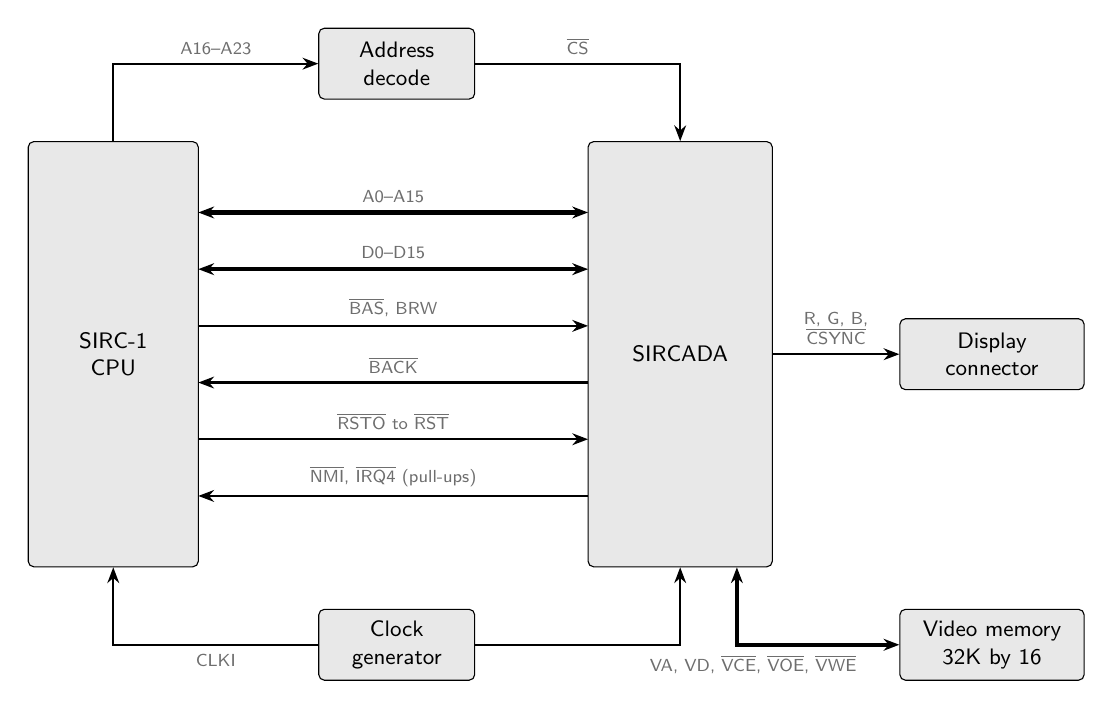
\begin{tikzpicture}[
			scale=0.9, transform shape,
			block/.style={draw, rounded corners=2pt, fill=sirclightgray, align=center, font=\small},
			sig/.style={-{Stealth[length=2mm]}, thick},
			bus/.style={{Stealth[length=2mm]}-{Stealth[length=2mm]}, ultra thick},
			note/.style={font=\scriptsize, text=sircgray, align=center}
		]
		\node[block, minimum width=2.4cm, minimum height=6.0cm] (cpu) at (0,0) {SIRC-1\\CPU};
		\node[block, minimum width=2.6cm, minimum height=6.0cm] (ppu) at (8.0,0) {SIRCADA};
		\node[block, minimum width=2.2cm, minimum height=1.0cm] (dec) at (4.0,4.1) {Address\\decode};
		\node[block, minimum width=2.2cm, minimum height=1.0cm] (clk) at (4.0,-4.1) {Clock\\generator};
		\node[block, minimum width=2.6cm, minimum height=1.0cm] (out) at (12.4,0) {Display\\connector};
		\node[block, minimum width=2.6cm, minimum height=1.0cm] (vram) at (12.4,-4.1) {Video memory\\32K by 16};
		% Lanes between the CPU and the device
		\draw[bus] (1.2,2.0) -- node[above, note]{A0--A15} (6.7,2.0);
		\draw[bus] (1.2,1.2) -- node[above, note]{D0--D15} (6.7,1.2);
		\draw[sig] (1.2,0.4) -- node[above, note]{\activelow{BAS}, BRW} (6.7,0.4);
		\draw[sig] (6.7,-0.4) -- node[above, note]{\activelow{BACK}} (1.2,-0.4);
		\draw[sig] (1.2,-1.2) -- node[above, note]{\activelow{RSTO} to \activelow{RST}} (6.7,-1.2);
		\draw[sig] (6.7,-2.0) -- node[above, note]{\activelow{NMI}, \activelow{IRQ4} (pull-ups)} (1.2,-2.0);
		% Address decode
		\draw[sig] (cpu.north) |- node[above, pos=0.75, note]{A16--A23} (dec.west);
		\draw[sig] (dec.east) -| node[above, pos=0.25, note]{\activelow{CS}} (ppu.north);
		% Clock
		\draw[sig] (clk.west) -| node[below, pos=0.25, note]{CLKI} (cpu.south);
		\draw[sig] (clk.east) -| (ppu.south);
		% Video
		\draw[sig] (ppu.east) -- node[above, note]{R, G, B,\\\activelow{CSYNC}} (out.west);
		% Video memory bus
		\draw[bus] ([xshift=0.8cm]ppu.south) |- node[below, pos=0.55, note]{VA, VD, \activelow{VCE}, \activelow{VOE}, \activelow{VWE}} (vram.west);
	\end{tikzpicture}
	\caption{The Video Device in a System}
	\label{fig:connections}
\end{figure}

\chapter{Memory Map and Bus Access}
\label{ch:memory-map}

\section{The Device Segment}

The video device occupies one segment of the CPU's address space, 65,536 words long. The segment is chosen by the
system; the reference virtual machine maps the device at segment \texttt{0x000C}, so a register at offset
\texttt{0x0002} is at the CPU address \texttt{0x000C\_0002}. This manual gives every address as an offset from the base
of the segment.

\begin{table}[H]
	\centering
	\begin{tabular}{llp{6.5cm}}
		\toprule
		\textbf{Offsets}                 & \textbf{Region} & \textbf{Notes}                                                                                           \\
		\midrule
		\texttt{0x0000}--\texttt{0x00FF} & Registers       & Offsets \texttt{0x0000}--\texttt{0x0018} are defined (Chapter~\ref{ch:registers}); the rest are open bus \\
		\texttt{0x0100}--\texttt{0x5FFF} & Unmapped        & Open bus                                                                                                 \\
		\texttt{0x6000}--\texttt{0x60FF} & Palette         & 256 entries, one word each (Section~\ref{sec:palette})                                                   \\
		\texttt{0x6100}--\texttt{0x7FFF} & Unmapped        & Open bus; see Section~\ref{sec:palette-edge}                                                             \\
		\texttt{0x8000}--\texttt{0xFFFF} & Video memory    & 32,768 words of tile data and tilemaps                                                                   \\
		\bottomrule
	\end{tabular}
	\caption{Video Device Memory Map}
	\label{tab:memory-map}
\end{table}

\section{Registers, Palette and Video Memory}

The \textbf{registers} control the device. They are described in Chapter~\ref{ch:registers}.

The \textbf{palette} holds 256 colours in a small, fast memory that the renderer reads once per pixel. It can be read
and written by the CPU at any time.

The \textbf{video memory} (VRAM) holds everything else: tile data, tilemaps and, when they are specified, sprite tile
data. It is 32,768 words, which is 64 KB. The device does not interpret VRAM in any fixed layout. Each background has a
base address register for its tilemap and another for its tile data, and any VRAM range may hold either. The only
constraint is that ranges the renderer reads must not overlap ranges the program expects to stay untouched.

An address in VRAM is written as its offset in the segment, so VRAM begins at \texttt{0x8000}. The base address
registers hold addresses in this form: a tilemap at the start of VRAM has the base address \texttt{0x8000}, not
\texttt{0x0000}.

\section{Access Rules}

A read of a register, a palette entry or a VRAM word returns the stored value. A write stores the value. A read of an
open bus offset returns zero and a write to one is ignored. The device never inserts a wait state: every access
completes in the cycle it is made, whether or not it takes effect (Section~\ref{sec:memory-vram-access}).

The Status register (offset \texttt{0x0017}) and the Vertical Line register (offset \texttt{0x0018}) are read-only; a
write to either is ignored.

\subsection{Access During Rendering}
\label{sec:memory-vram-access}

The renderer reads video memory in the visible lines, and in the horizontal blanking interval too: the sprites of the
next line are fetched there (Chapter~\ref{ch:sprites}). So video memory and the sprite table are available to the CPU
only in vertical blanking, the lines after the last visible line (Chapter~\ref{ch:timing}), or while the picture is
turned off (\texttt{GD} in the Base Configuration register is 1), when the device makes no reads at all:

\begin{itemize}
	\item A write to video memory or to the sprite table at any other time is ignored, and a read returns zero. At reset
	      \texttt{GD} is 1, so a program can load video memory straight away and then clear \texttt{GD}.
	\item The palette and the registers can be read and written at any time. A palette write changes the colour of the pixels
	      drawn after it, which allows a palette change in the middle of the picture. A register write takes effect when the
	      device next samples that register, normally at the start of the next line (Chapters~\ref{ch:mode2} and~\ref{ch:mode3}).
\end{itemize}

\subsection{The Palette Boundary}
\label{sec:palette-edge}

The palette occupies 256 words, \texttt{0x6000}--\texttt{0x60FF}. The offset \texttt{0x6100} and the rest of the range
up to \texttt{0x7000} are open bus.

\section{Planning a VRAM Layout}

Nothing fixes where tile data and tilemaps live, so a program chooses. One arrangement puts the tile set at the bottom
of VRAM and the tilemaps at the top, leaving room for the tile set to grow:

\begin{table}[H]
	\centering
	\begin{tabular}{lll}
		\toprule
		\textbf{Contents}    & \textbf{Offsets}       & \textbf{Size}     \\
		\midrule
		Tile set (Mode 1)    & \texttt{0x8000} and up & 16 words per tile \\
		Background 1 tilemap & \texttt{0xF000}        & 1024 words        \\
		Background 2 tilemap & \texttt{0xF400}        & 1024 words        \\
		Background 3 tilemap & \texttt{0xF800}        & 1024 words        \\
		\bottomrule
	\end{tabular}
	\caption{An Example Mode 1 VRAM Layout}
	\label{tab:vram-layout}
\end{table}

A tilemap is a 32 by 32 table of one-word entries, so it takes 1024 words. A Mode 1 tile of 8 by 8 pixels at 4 bits per
pixel takes 16 words; a Mode 2 tile of 16 by 16 texels takes 64 words (Section~\ref{sec:m2-tile-format}). VRAM can
therefore hold at most 2048 Mode 1 tiles or 512 Mode 2 tiles, before any tilemap is placed in it.

\chapter{Registers}
\label{ch:registers}

\section{Register Map}

The registers occupy the first words of the device segment. Every defined register is 16 bits wide and is read and
written a word at a time.

\begin{table}[H]
	\centering
	\begin{tabular}{lllp{5.2cm}}
		\toprule
		\textbf{Offset}                  & \textbf{Name}     & \textbf{Access} & \textbf{Description}                                     \\
		\midrule
		\texttt{0x0000}                  & \texttt{CONFIG}   & R/W             & Base configuration: mode, layer disables, brightness     \\
		\texttt{0x0001}                  & \texttt{TILESIZE} & R/W             & Tile and tilemap sizes                                   \\
		\texttt{0x0002}                  & \texttt{B1MAP}    & R/W             & Background 1 tilemap address                             \\
		\texttt{0x0003}                  & \texttt{B2MAP}    & R/W             & Background 2 tilemap address                             \\
		\texttt{0x0004}                  & \texttt{B3MAP}    & R/W             & Background 3 tilemap address                             \\
		\texttt{0x0005}                  & ---               & Reserved        &                                                          \\
		\texttt{0x0006}                  & \texttt{B1TILES}  & R/W             & Background 1 tile data address                           \\
		\texttt{0x0007}                  & \texttt{B2TILES}  & R/W             & Background 2 tile data address                           \\
		\texttt{0x0008}                  & \texttt{B3TILES}  & R/W             & Background 3 tile data address                           \\
		\texttt{0x0009}                  & ---               & Reserved        &                                                          \\
		\texttt{0x000A}                  & \texttt{B1SCRX}   & R/W             & Background 1 horizontal scroll                           \\
		\texttt{0x000B}                  & \texttt{B2SCRX}   & R/W             & Background 2 horizontal scroll                           \\
		\texttt{0x000C}                  & \texttt{B3SCRX}   & R/W             & Background 3 horizontal scroll                           \\
		\texttt{0x000D}                  & ---               & Reserved        &                                                          \\
		\texttt{0x000E}                  & \texttt{B1SCRY}   & R/W             & Background 1 vertical scroll                             \\
		\texttt{0x000F}                  & \texttt{B2SCRY}   & R/W             & Background 2 vertical scroll                             \\
		\texttt{0x0010}                  & \texttt{B3SCRY}   & R/W             & Background 3 vertical scroll                             \\
		\texttt{0x0011}                  & \texttt{INTCTL}   & R/W             & Interrupt enables                                        \\
		\texttt{0x0012}                  & \texttt{B1PAL}    & R/W             & Background 1 palette configuration                       \\
		\texttt{0x0013}                  & \texttt{B2PAL}    & R/W             & Background 2 palette configuration                       \\
		\texttt{0x0014}                  & \texttt{B3PAL}    & R/W             & Background 3 palette configuration                       \\
		\texttt{0x0015}                  & \texttt{LINE}     & R/W             & Line-compare interrupt line; a write acknowledges        \\
		\texttt{0x0016}                  & \texttt{STILES}   & R/W             & Sprite tile data address                                 \\
		\texttt{0x0017}                  & \texttt{STATUS}   & R               & Version, output mode, sprite overflow, vertical blanking \\
		\texttt{0x0018}                  & \texttt{VLINE}    & R               & Current line                                             \\
		\texttt{0x0019}--\texttt{0x00FF} & ---               & Open bus        & Reads zero, writes ignored                               \\
		\bottomrule
	\end{tabular}
	\caption{Register Map}
	\label{tab:register-map}
\end{table}

The register names are those of this manual. Software must not write the reserved registers. The registers are laid out
in groups of three backgrounds followed by one reserved slot, so a register for background $n$ is at the group's base
plus $n - 1$.

\section{Base Configuration Register}
\label{sec:reg-base-config}

\begin{figure}[H]
	\centering
	\begin{bytefield}[bitwidth=2em]{16}
		\bitheader{0-15} \\
		\bitbox{1}{GD} &
		\bitbox{1}{B1D} &
		\bitbox{1}{B2D} &
		\bitbox{1}{B3D} &
		\bitbox{1}{} &
		\bitbox{1}{S1D} &
		\bitbox{1}{S2D} &
		\bitbox{1}{S3D} &
		\bitbox{1}{\footnotesize SHD} &
		\bitbox{4}{BRT} &
		\bitbox{3}{MODE}
	\end{bytefield}
	\caption{Base Configuration Register (\texttt{CONFIG}, Offset \texttt{0x0000})}
	\label{fig:reg-config}
\end{figure}

\begin{table}[H]
	\centering
	\begin{tabular}{llp{7.5cm}}
		\toprule
		\textbf{Bits} & \textbf{Field}                           & \textbf{Meaning}                                                                                                                                                                             \\
		\midrule
		15            & \texttt{GD}                              & Graphics disable (forced blank): when 1 the picture is black and the device makes no reads, so video memory and the sprite table can be accessed at any time. 1 at reset                     \\
		14, 13, 12    & \texttt{B1D}, \texttt{B2D}, \texttt{B3D} & Disable background 1, 2, 3 when 1 (Section~\ref{sec:m2-layers})                                                                                                                              \\
		11            & ---                                      & Reserved                                                                                                                                                                                     \\
		10, 9, 8      & \texttt{S1D}, \texttt{S2D}, \texttt{S3D} & Disable sprite layer 1, 2, 3 when 1 (Chapter~\ref{ch:sprites})                                                                                                                               \\
		7             & \texttt{SHD}                             & Sprite shadow enable: when 1, value 15 of sprite palette 7 is a shadow (Section~\ref{sec:sprite-shadow}); 0 at reset                                                                         \\
		6--3          & \texttt{BRT}                             & Screen brightness: each colour channel of the final picture is multiplied by $(\texttt{BRT} + 1)/16$, so 15 is full brightness and 0 nearly black. \texttt{GD} blanks the picture completely \\
		2--0          & \texttt{MODE}                            & Video mode: 0 for Mode 1, 1 for Mode 2, 2 for Mode 3, others reserved                                                                                                                        \\
		\bottomrule
	\end{tabular}
	\caption{Base Configuration Register Fields}
	\label{tab:reg-config-fields}
\end{table}

The \texttt{MODE} field is sampled at the first cycle of each line, so a change takes effect at the start of the next
line. Software should change mode during vertical blanking.

\section{Tile Size Register}
\label{sec:reg-tilesize}

\begin{figure}[H]
	\centering
	\begin{bytefield}[bitwidth=2em]{16}
		\bitheader{0-15} \\
		\bitbox{1}{B1S} &
		\bitbox{1}{B2S} &
		\bitbox{1}{B3S} &
		\bitbox{1}{} &
		\bitbox{1}{S1S} &
		\bitbox{1}{S2S} &
		\bitbox{1}{S3S} &
		\bitbox{1}{} &
		\bitbox{1}{B1X} &
		\bitbox{1}{B2X} &
		\bitbox{1}{B3X} &
		\bitbox{1}{} &
		\bitbox{1}{B1Y} &
		\bitbox{1}{B2Y} &
		\bitbox{1}{B3Y} &
		\bitbox{1}{}
	\end{bytefield}
	\caption{Tile Size Register (\texttt{TILESIZE}, Offset \texttt{0x0001})}
	\label{fig:reg-tilesize}
\end{figure}

\begin{table}[H]
	\centering
	\begin{tabular}{llp{7.5cm}}
		\toprule
		\textbf{Bits} & \textbf{Field}                           & \textbf{Meaning}                                                                          \\
		\midrule
		15, 14, 13    & \texttt{B1S}, \texttt{B2S}, \texttt{B3S} & Orthogonal background tile size: 0 for 8 by 8, 1 for 16 by 16 (Section~\ref{sec:flat-16}) \\
		11, 10, 9     & \texttt{S1S}, \texttt{S2S}, \texttt{S3S} & Sprite tile size, same encoding                                                           \\
		7, 6, 5       & \texttt{B1X}, \texttt{B2X}, \texttt{B3X} & Tilemap width: 0 for one screen of 32 entries, 1 for two (Section~\ref{sec:tilemap-size}) \\
		3, 2, 1       & \texttt{B1Y}, \texttt{B2Y}, \texttt{B3Y} & Tilemap height: 0 for one screen of 32 entries, 1 for two                                 \\
		12, 8, 4, 0   & ---                                      & Reserved                                                                                  \\
		\bottomrule
	\end{tabular}
	\caption{Tile Size Register Fields}
	\label{tab:reg-tilesize-fields}
\end{table}

An \emph{orthogonal} background is an ordinary background of square tiles in rows and columns, as opposed to an
isometric one. The word is used for all of them: the three backgrounds of Mode 1, the two of Mode 3 and the status
layer of Mode 2. Orthogonal backgrounds scroll, except for the status layer of Mode 2. The tile size bits
\texttt{B1S}--\texttt{B3S} apply to orthogonal backgrounds, that is, to all three backgrounds in Mode 1 and to
backgrounds 1 and 2 in Mode 3, but not to the status layer, which always uses 8 by 8 tiles. The tilemap size bits apply
to orthogonal and isometric backgrounds. Isometric backgrounds always use 16 by 16 texel tiles and ignore the tile size
bits (Section~\ref{sec:m2-restrictions}).

\section{Tilemap and Tile Data Address Registers}

\texttt{B1MAP}--\texttt{B3MAP} hold the word address of the first entry of the background's tilemap. \texttt{B1TILES}--\texttt{B3TILES}
hold the word address of the first word of tile number 0 of its tile data. Both are full offsets within the segment, so
a value for VRAM is at least \texttt{0x8000} (Chapter~\ref{ch:memory-map}). All 16 bits are significant. The renderer
adds the offset of an entry or tile to the base with 16-bit wraparound.

\texttt{STILES} holds the sprite tile data address (Chapter~\ref{ch:sprites}).

\section{Scroll Registers}

\begin{figure}[H]
	\centering
	\begin{bytefield}[bitwidth=2em]{16}
		\bitheader{0-15} \\
		\bitbox{6}{} &
		\bitbox{10}{SCROLL}
	\end{bytefield}
	\caption{Scroll Registers (\texttt{B1SCRX}--\texttt{B3SCRY})}
	\label{fig:reg-scroll}
\end{figure}

Bits 9--0 hold the scroll amount, 0 to 1023, in pixels. Bits 15--10 are reserved. The amount moves the background's
view of its map: increasing \texttt{SCRX} moves the picture to the left, and increasing \texttt{SCRY} moves it up.

Every background of every mode scrolls. The amounts are sampled once per line, as the chapter of each mode describes.

\section{Palette Configuration Registers}
\label{sec:reg-palette}

\begin{figure}[H]
	\centering
	\begin{bytefield}[bitwidth=2em]{16}
		\bitheader{0-15} \\
		\bitbox{8}{OFFSET} &
		\bitbox{6}{} &
		\bitbox{2}{SIZE}
	\end{bytefield}
	\caption{Palette Configuration Registers (\texttt{B1PAL}--\texttt{B3PAL})}
	\label{fig:reg-pal}
\end{figure}

\begin{table}[H]
	\centering
	\begin{tabular}{llp{7.5cm}}
		\toprule
		\textbf{Bits} & \textbf{Field}  & \textbf{Meaning}                                                       \\
		\midrule
		15--8         & \texttt{OFFSET} & Palette entry added to every colour address of the background          \\
		7--3          & ---             & Reserved                                                               \\
		2             & \texttt{T2}     & 2-bit tiles (Sections~\ref{sec:m2-two-bit} and~\ref{sec:flat-two-bit}) \\
		1--0          & \texttt{SIZE}   & Colours per palette: 0 for 4, 1 for 8, 2 for 16, 3 for 32              \\
		\bottomrule
	\end{tabular}
	\caption{Palette Configuration Register Fields}
	\label{tab:reg-pal-fields}
\end{table}

Section~\ref{sec:palette-select} explains how \texttt{OFFSET} and \texttt{SIZE} combine with a tilemap entry's palette
selection to choose a palette entry. 4-bit tile data uses sizes of 16 colours or fewer.

\section{Status Register}

\begin{figure}[H]
	\centering
	\begin{bytefield}[bitwidth=2em]{16}
		\bitheader{0-15} \\
		\bitbox{8}{} &
		\bitbox{1}{VBL} &
		\bitbox{1}{LIP} &
		\bitbox{1}{SOV} &
		\bitbox{1}{OUT} &
		\bitbox{4}{VER}
	\end{bytefield}
	\caption{Status Register (\texttt{STATUS}, Offset \texttt{0x0017})}
	\label{fig:reg-status}
\end{figure}

\texttt{VER}, bits 3--0, is the version of the device, which is 1. \texttt{OUT}, bit 4, is the output mode: 0 for NTSC and
1 for PAL. Both are fixed when the device is made. \texttt{SOV}, bit 5, is the sprite overflow flag: it is set when any
line of the frame had more than 32 sprites (Section~\ref{sec:sprite-budget}), and cleared at the start of line 0 of the
next frame, so a program reads it in vertical blanking. \texttt{LIP}, bit 6, is set while a line-compare interrupt is
pending (Section~\ref{sec:line-interrupt}). \texttt{VBL}, bit 7, is set while the beam is in vertical blanking, from the first cycle
of line 224 to the last cycle of the last line of the frame, and is clear in lines 0 to 223; it is the flag a program
polls to know that video memory is open (Section~\ref{sec:memory-vram-access}). Bits 15--8 are reserved. The register is read-only.

\section{Vertical Line Register}
\label{sec:reg-vline}

\texttt{VLINE}, offset \texttt{0x0018}, holds in bits 8--0 the number of the line the beam is on: 0 to 261 on NTSC and 0 to 311 on
PAL. It changes at the first cycle of each line, the cycle at which a line-compare interrupt for that line is raised, and
bits 15--9 read as zero. The register is read-only. A program reads it to find where in the frame it is, and
reads it twice, or compares it with \texttt{LINE}, when a line may have passed between two accesses.

\section{Line Compare Register}
\label{sec:reg-line}

\texttt{LINE} holds, in bits 8--0, the number of the line at which the line-compare interrupt fires when \texttt{LIE} is set
in the Interrupt Control register (Section~\ref{sec:line-interrupt}). Bits 15--9 are reserved. A write to \texttt{LINE}, of
any value, also acknowledges a pending line-compare interrupt.

\section{Interrupt Control Register}
\label{sec:reg-intctl}

\begin{figure}[H]
	\centering
	\begin{bytefield}[bitwidth=2em]{16}
		\bitheader{0-15} \\
		\bitbox{14}{} &
		\bitbox{1}{LIE} &
		\bitbox{1}{VIE}
	\end{bytefield}
	\caption{Interrupt Control Register (\texttt{INTCTL}, Offset \texttt{0x0011})}
	\label{fig:reg-intctl}
\end{figure}

\begin{table}[H]
	\centering
	\begin{tabular}{llp{7.5cm}}
		\toprule
		\textbf{Bits} & \textbf{Field} & \textbf{Meaning}                                                                                           \\
		\midrule
		15--2         & ---            & Reserved                                                                                                   \\
		1             & \texttt{LIE}   & Line interrupt enable: when 1, the line-compare interrupt can be raised (Section~\ref{sec:line-interrupt}) \\
		0             & \texttt{VIE}   & Vertical sync interrupt enable: when 1, the device raises the NMI at the start of vertical blanking        \\
		\bottomrule
	\end{tabular}
	\caption{Interrupt Control Register Fields}
	\label{tab:reg-intctl-fields}
\end{table}

Both bits are 0 at reset, so no interrupt is raised until the program has set up its handlers.

\section{Reset State}
\label{sec:reset}

At reset the device is blank and every register is zero, except as follows:

\begin{table}[H]
	\centering
	\begin{tabular}{lll}
		\toprule
		\textbf{Register} & \textbf{Value at reset} & \textbf{Meaning}                                                      \\
		\midrule
		\texttt{CONFIG}   & \texttt{0x8078}         & \texttt{GD} = 1 (picture blank), \texttt{BRT} = 15, \texttt{MODE} = 0 \\
		\bottomrule
	\end{tabular}
	\caption{Registers with a Non-Zero Reset Value}
	\label{tab:reset}
\end{table}

The contents of video memory, the palette and the sprite table are undefined at reset. A program must initialise
whatever it uses, and then clear \texttt{GD}, before the picture is shown. A program should hide every sprite it does
not use (layer 3) before it clears \texttt{GD}.


\chapter{Data Formats}
\label{ch:data-formats}

\section{Colour}
\label{sec:colour}

A colour is a 16-bit word with 5 bits for each of red, green and blue. Bit 15 is a reserved flag.

\begin{figure}[H]
	\centering
	\begin{bytefield}[bitwidth=1.5em]{16}
		\bitheader{0-15} \\
		\bitbox{1}{F} &
		\bitbox{5}{R} &
		\bitbox{5}{G} &
		\bitbox{5}{B}
	\end{bytefield}
	\caption{Colour Format}
	\label{fig:colour}
\end{figure}

Each 5-bit channel drives the converter of its colour output (Chapter~\ref{ch:package}), which has 32 evenly spaced
levels from black to full scale. Channel value 31 is full scale, so a pixel of 31 in every channel is full-scale white.

\section{The Palette}
\label{sec:palette}

The palette holds 256 colours at offsets \texttt{0x6000}--\texttt{0x60FF} (Chapter~\ref{ch:memory-map}). Every pixel of
every background is a palette lookup. Palette entry 0 is special in one way: it is the backdrop, the colour shown where
no layer has a visible pixel.

\section{Tile Data}
\label{sec:tile-data}

A tile is a small square image of 4-bit pixels, each of which is a number from 0 to 15. The value 0 is transparent: the
pixel shows whatever is behind it. The values 1--15 select a colour through the palette
(Section~\ref{sec:palette-select}).

\subsection{Mode 1 Tile Layout}
\label{sec:m1-tile-layout}

Four pixels fill one 16-bit word, with the leftmost pixel in the most significant nibble.

\begin{figure}[H]
	\centering
	\begin{bytefield}[bitwidth=1.5em]{16}
		\bitheader{0-15} \\
		\bitbox{4}{P1} &
		\bitbox{4}{P2} &
		\bitbox{4}{P3} &
		\bitbox{4}{P4}
	\end{bytefield}
	\caption{Four Pixels of Tile Data}
	\label{fig:tile-word}
\end{figure}

An 8 by 8 tile is stored as eight rows of two words each, top row first, so it occupies 16 words. The word for pixels
$4h$ to $4h + 3$ of row $r$ of tile $t$ is at the tile data base address plus $16t + 2r + h$, where $h$ is 0 for the
left half of the row and 1 for the right half. A 16 by 16 tile is described in Section~\ref{sec:flat-16}.

\subsection{Mode 2 Tile Layout}

Mode 2 stores a 16 by 16 texel tile in a different arrangement, described in Section~\ref{sec:m2-tile-format}. It takes
64 words, the same as a 16 by 16 tile would in the row-by-row layout, but the words are not rows.

\subsection{16 by 16 Orthogonal Tiles}
\label{sec:flat-16}

An orthogonal background whose tile size bit (Section~\ref{sec:reg-tilesize}) is 1 uses 16 by 16 tiles. A 16 by 16 tile
is stored as four 8 by 8 quadrants in the order top left, top right, bottom left, bottom right, each laid out as in
Section~\ref{sec:m1-tile-layout}, so a tile is 64 words. For the pixel in column $c$ and row $r$ of tile $t$ the word
is at

\begin{center}
	\texttt{tile data base + 64 $\times$ tile number + 16 $\times$ quadrant + 2 $\times$ (row mod 8) + half}
\end{center}

where the quadrant is $2\lfloor r/8 \rfloor + \lfloor c/8 \rfloor$ and the half is $\lfloor (c \bmod 8)/4 \rfloor$. A
2-bit 16 by 16 tile is four quadrants of 8 words, 32 words, with the word at \texttt{base + 32 $\times$ tile + 8
	$\times$ quadrant + (row mod 8)}. A tile of 64 words is the same size as an isometric tile, so one tile number
addresses either. With 16 by 16 tiles a 32 by 32 tilemap covers 512 by 512 pixels. Each background chooses its own tile
size, and backgrounds of different tile sizes need no further rule: each is fetched independently.

\subsection{Flipping Orthogonal Tiles}

When the \texttt{H} bit of an orthogonal tilemap entry is set, the tile is mirrored left to right: pixel column $c$ is
read from column $w - 1 - c$ of the tile, where $w$ is 8 or 16. When \texttt{V} is set, row $r$ is read from row $w - 1
	- r$. The device reads the mirrored word and reverses the order of its pixels.

\subsection{2-Bit Orthogonal Tiles}
\label{sec:flat-two-bit}

A background whose \texttt{T2} bit (Section~\ref{sec:reg-palette}) is set uses 2-bit tiles. An 8 by 8 orthogonal tile
is then 8 words, one for each row, holding the row's eight pixels with the leftmost in bits 15--14:

\begin{center}
	\texttt{tile data base + 8 $\times$ tile number + row}
\end{center}

Value 0 is transparent, so a pixel has three colours. A word covers eight pixels, so the device reads it for every
second group of four. 2-bit tiles apply to every orthogonal background and to the status layer. Isometric 2-bit tiles
have a layout of their own (Section~\ref{sec:m2-two-bit}).

\section{Tilemap Entries}
\label{sec:tilemap-entry}

A tilemap is a table of one-word entries, 32 entries to a row and 32 rows, stored row by row. An entry names a tile and
how it is drawn.

\begin{figure}[H]
	\centering
	\begin{bytefield}[bitwidth=1.5em]{16}
		\bitheader{0-15} \\
		\bitbox{1}{V} &
		\bitbox{1}{H} &
		\bitbox{1}{P} &
		\bitbox{3}{PAL} &
		\bitbox{10}{TILE}
	\end{bytefield}
	\caption{Tilemap Entry}
	\label{fig:tilemap-entry}
\end{figure}

\begin{table}[H]
	\centering
	\begin{tabular}{llp{7.5cm}}
		\toprule
		\textbf{Bits} & \textbf{Field} & \textbf{Meaning}                                                                                                                                     \\
		\midrule
		15            & \texttt{V}     & Flip the tile vertically on an orthogonal layer (Section~\ref{sec:flat-16}); darkens the tile in an isometric layer (Section~\ref{sec:m2-shading})   \\
		14            & \texttt{H}     & Flip the tile horizontally on an orthogonal layer; lightens the tile in an isometric layer                                                           \\
		13            & \texttt{P}     & Priority: 1 puts the tile in front of everything, sprite layer 1 included; 0 leaves its layer in the order S1, B1, S2, B2, S3, B3 (and B4 in Mode 1) \\
		12--10        & \texttt{PAL}   & Palette selection, 0 to 7 (Section~\ref{sec:palette-select})                                                                                         \\
		9--0          & \texttt{TILE}  & Tile number, 0 to 1023, counted from the background's tile data base address                                                                         \\
		\bottomrule
	\end{tabular}
	\caption{Tilemap Entry Fields}
	\label{tab:tilemap-entry-fields}
\end{table}

Tile numbers can reach 1023, but VRAM is not that large for every tile size: 64-word tiles stop at 512 in a VRAM with
nothing else in it (Chapter~\ref{ch:memory-map}). A tile number whose data lies past the end of the address space wraps
at 16 bits.

\section{Tilemap Sizes}
\label{sec:tilemap-size}

A tilemap is made of screens of 32 by 32 entries, stored row by row, 1,024 words each. The width bit \texttt{BnX} and
the height bit \texttt{BnY} of the Tile Size register (Section~\ref{sec:reg-tilesize}) double the map across or down:

\begin{center}
	\begin{tabular}{ccl}
		\toprule
		\texttt{BnX} & \texttt{BnY} & Map                                                 \\
		\midrule
		0            & 0            & One screen, 32 by 32 entries                        \\
		1            & 0            & Two screens side by side, 64 by 32: A B             \\
		0            & 1            & Two screens one above the other, 32 by 64: A over B \\
		1            & 1            & Four screens, 64 by 64: A B over C D                \\
		\bottomrule
	\end{tabular}
\end{center}

The screens are in memory in the order A, B, C, D, starting at the tilemap base. For the entry in column $c$ and row
$r$ of a map $W$ entries wide and $H$ high (both after wrapping, $c \bmod W$ and $r \bmod H$), the address is

\begin{center}
	\texttt{tilemap base + 1024 $\times$ screen + 32 $\times$ (r mod 32) + (c mod 32)}
\end{center}

where the screen is $\lfloor r/32 \rfloor \cdot (W/32) + \lfloor c/32 \rfloor$. A map wraps at its size. The tilemap
sizes apply to orthogonal backgrounds, where an entry is a tile, and to isometric backgrounds, where an entry is a cell
(Section~\ref{sec:m2-tilemap}).

\section{Palette Selection}
\label{sec:palette-select}

A background pixel with a non-zero value $v$ in a tile whose entry has palette selection $s$ reads palette entry
\[
	\text{entry} = ((s \ll k) + \texttt{OFFSET} + v) \bmod 256,
\]
where \texttt{OFFSET} and $k$ come from the background's palette configuration register
(Section~\ref{sec:reg-palette}): $k$ is 2, 3, 4 or 5 for \texttt{SIZE} values 0, 1, 2 and 3, that is, for palettes of
4, 8, 16 or 32 colours. The sum wraps at 8 bits. A pixel whose value is 0 is transparent and reads no palette entry.

With 16-colour palettes, \texttt{OFFSET} 0 and a selection of 3, the value 5 reads palette entry 53. The eight
selections therefore pick eight palettes of 16 colours, 128 palette entries in all, starting at the offset.

\section{Compositing Rule}
\label{sec:compositing}

Layers are combined pixel by pixel. For each screen pixel the device takes the first layer, in front-to-back order,
whose pixel value is not 0, and shows the palette entry that pixel selects. If every layer is transparent, the device
shows palette entry 0. There is no blending: a pixel is either transparent or fully opaque.

The front-to-back order of the layers is S1, B1, S2, B2, S3, B3, B4 in Mode 1, the same without B4 in Mode 3, and S1,
B1, S2, B2, S3 with a status layer in Mode 2; see Sections~\ref{sec:m1-priority} and~\ref{sec:m2-layers}. A tile with
its priority bit set is in front of everything.

\chapter{Mode 1: Orthogonal Backgrounds}
\label{ch:mode1}

\section{Overview}

Mode 1 is the device's conventional mode, the one it is in at reset. It draws up to three backgrounds of square tiles
laid out in rows and columns, and three layers of sprites. The tiles of a background are 4 bits per pixel, or 2 bits
when its \texttt{T2} bit is set (Section~\ref{sec:flat-two-bit}).

\section{Backgrounds}

Each background is a tilemap (Section~\ref{sec:tilemap-size}), 32 by 32 entries by default, and a set of tiles of 8 by
8 or 16 by 16 pixels (Section~\ref{sec:tile-data}). Each of the three chooses its own tile size and tilemap size, so a
background covers from 256 by 256 pixels (8 by 8 tiles, one screen) to 1024 by 1024 (16 by 16 tiles, four screens), and
the 256 by 224 picture is a window onto it. Each background also has its own scroll registers and palette
configuration.

For the pixel at screen column $x$ and line $y$, the renderer reads, for a background with scroll $(s_x, s_y)$ and
tiles $w$ pixels square, the tilemap entry in column $\lfloor (x + s_x)/w \rfloor$ and row $\lfloor (y + s_y)/w
	\rfloor$, both taken modulo the size of the map, and then the word of tile data holding the pixel
(Sections~\ref{sec:m1-tile-layout} and~\ref{sec:flat-16}). It does this for all three backgrounds at once.

\subsection{Scrolling}
\label{sec:m1-scrolling}

Scrolling works as it does for the orthogonal backgrounds of Mode 3 (Section~\ref{sec:m3-scrolling}): the scroll
registers are sampled once per line, groups of four pixels are aligned to the plane, a window of two groups with an
offset of $s_x \bmod 4$ gives fine scrolling, and a map wraps at its size.

\section{Programming Mode 1}

\begin{enumerate}
	\item Write the palette, the tile data and the tilemaps into video memory, in vertical blanking or while \texttt{GD} is 1.
	\item Write the \texttt{TILESIZE} register with the tile size and tilemap size of each background.
	\item Write the tilemap address, tile data address and palette configuration registers of each background in use.
	\item Write the Base Configuration register with \texttt{MODE} = 0, and with the disable bit of each unused background set.
	\item Each frame, during vertical blanking, write the scroll registers and any tilemap entries that have changed.
\end{enumerate}

\section{Priority and Compositing}
\label{sec:m1-priority}

The front-to-back order of the layers is sprite layer 1, background 1, sprite layer 2, background 2, sprite layer 3,
background 3.

Within a layer the compositing rule of Section~\ref{sec:compositing} applies: a pixel with value 0 is transparent. A
tile whose priority bit is set is in front of everything, sprite layer 1 included; its pixels of value 0 are still
transparent.

\section{Fetch Schedule}

The device reads video memory once per PPU cycle, and draws four pixels in eight PPU cycles, so every group of four
pixels has eight fetch slots. Mode 1 uses them as follows:

\begin{table}[H]
	\centering
	\begin{tabular}{cl}
		\toprule
		\textbf{Slot} & \textbf{Fetch}              \\
		\midrule
		0             & Background 1 tilemap entry  \\
		1             & Background 2 tilemap entry  \\
		2             & Background 3 tilemap entry  \\
		3             & Background 1 tile data word \\
		4             & Background 2 tile data word \\
		5             & Background 3 tile data word \\
		6, 7          & Not used                    \\
		\bottomrule
	\end{tabular}
	\caption{Mode 1 Fetch Slots per Group of Four Pixels}
	\label{tab:m1-slots}
\end{table}

An 8 by 8 tile is eight pixels wide, so the tilemap entries are fetched twice for each tile, once for each group of
four, and the device does not keep an entry for the second group. The fetched pixels are combined into four finished
pixels at the start of the next group (Chapter~\ref{ch:timing}).

\chapter{Mode 2: Isometric Backgrounds}
\label{ch:mode2}

\section{Overview}

Mode 2 draws two backgrounds as a 2:1 isometric ground plane. Each background is an ordinary map of square tiles, but
the device does not draw the map in rows and columns. It samples the map along diagonals so that every square tile
appears as a diamond, 32 pixels wide and 16 pixels high, and the whole map appears as the flat, tilted landscape of a
strategy or simulation game.

\begin{description}
	\item[Selected by:] \texttt{MODE} = 1 in the Base Configuration register.
	\item[Layers:] Two isometric backgrounds, 1 (front) and 2 (back), and an orthogonal status layer, background 3. Sprites are
	      drawn as in Mode 1 (Chapter~\ref{ch:sprites}).
	\item[Tiles:] 16 by 16 texels, 4 bits per texel, 64 words each, in the staircase layout of Section~\ref{sec:m2-tile-format}.
	\item[Map:] One 32 by 32 tilemap per background, wrapping in both directions.
\end{description}

\subsection{What the Mode Is For}

Mode 2 is a specialised mode. It is good at one picture, a large flat map seen from above at an angle, with
pixel-smooth scrolling and a map that is the game's own grid. Transport and city-building games are of this kind.

It is poor at nearly everything else, and the reasons come from the same design decision that makes it good at its job:

\begin{itemize}
	\item Every screen pixel belongs to exactly one tile of a layer. A tile cannot overhang its neighbours the way a sprite can,
	      so buildings, trees and vehicles are not drawn by the tile hardware. They are sliced into many tiles by a tool
	      (Section~\ref{sec:m2-authoring}) or drawn by sprites.
	\item Each group of four pixels needs a word of tile data, and sometimes two, because neighbouring pixels sit on different
	      rows of the tile and the group can lie on the edge of two tiles. That keeps most of the device's fetch bandwidth in
	      use, so the mode has two isometric backgrounds instead of three and no slot reserved for sprites
	      (Section~\ref{sec:m2-fetch}).
	\item The view cannot be rotated by a register. Art is drawn for one facing.
\end{itemize}

Programs that want side-scrolling backgrounds, parallax or many moving objects belong in Mode 1.

\section{Geometry}
\label{sec:m2-geometry}

Mode 2 works in a \emph{plane}: the screen pixel $(x, y)$ of a background plus that background's scroll, so the plane
pixel is $(X, Y) = (x + \texttt{SCRX},\, y + \texttt{SCRY})$. Plane pixel $(X, Y)$ shows the map texel $(u, v)$ given
by
\begin{align*}
	u & = Y + \lfloor X / 2 \rfloor,       \\
	v & = Y - \lfloor (X + 1) / 2 \rfloor,
\end{align*}
and the texel belongs to the tilemap cell $(c_u, c_v) = (\lfloor u / 16 \rfloor, \lfloor v / 16 \rfloor)$, with both
indices taken modulo 32, at position $(u \bmod 16, v \bmod 16)$ inside its tile. The formula uses two adders and no
multiplier. One step to the right moves half a texel along $u$ and half a texel back along $v$; one step down moves one
texel along each.

Three properties of the mapping matter:

\begin{itemize}
	\item $u - v = X$ for every pixel. This is what makes four neighbouring pixels a staircase of four texels
	      (Section~\ref{sec:m2-tile-format}).
	\item It is a bijection. Every texel of a tile is shown by exactly one pixel, so a tile has as many pixels as texels, 256,
	      and nothing is lost or repeated when an orthogonal tile is drawn as a diamond. An artist's diamond can be unwrapped
	      into a square tile and shown again without any change (Section~\ref{sec:m2-authoring}).
	\item The picture is a 2:1 isometric (dimetric) view. It is not a 45 degree rotation of the tile, which would need a
	      multiplication by 0.707 and would not be a bijection.
\end{itemize}

\subsection{The Diamond Footprint}

The pixels that show one tile form a diamond. Its top pixel is the plane pixel
\[
	(X, Y) = (16(c_u - c_v),\; 8(c_u + c_v)),
\]
which shows texel $(0, 0)$ of the tile. Table~\ref{tab:m2-footprint} gives the rows of the footprint; each is centred
on the column of the top pixel. The diamond is 31 pixels wide at its widest and 16 pixels high, which is why the
lattice is described as a 32 by 16 diamond: the neighbouring cell $(c_u + 1, c_v)$ has its top pixel 16 pixels to the
right and 8 pixels down, and the cell $(c_u, c_v + 1)$ has it 16 pixels to the left and 8 pixels down.

\begin{table}[H]
	\centering
	\begin{tabular}{rrr@{\hspace{2.5em}}rrr}
		\toprule
		\textbf{Row} & \textbf{Half-width} & \textbf{Width} & \textbf{Row} & \textbf{Half-width} & \textbf{Width} \\
		\midrule
		0            & 0                   & 1              & 8            & 15                  & 31             \\
		1            & 2                   & 5              & 9            & 13                  & 27             \\
		2            & 4                   & 9              & 10           & 11                  & 23             \\
		3            & 6                   & 13             & 11           & 9                   & 19             \\
		4            & 8                   & 17             & 12           & 7                   & 15             \\
		5            & 10                  & 21             & 13           & 5                   & 11             \\
		6            & 12                  & 25             & 14           & 3                   & 7              \\
		7            & 14                  & 29             & 15           & 1                   & 3              \\
		\bottomrule
	\end{tabular}
	\caption{Rows of a Tile's Diamond Footprint (256 Pixels in All)}
	\label{tab:m2-footprint}
\end{table}

The footprint is not quite symmetric from top to bottom: the top row is one pixel and the bottom row is three. This is
the shape that makes the mapping a bijection, and it is the shape the diamonds of a map tessellate in. A visible area
of 256 by 224 pixels shows 224 tiles' worth of pixels.

\section{Tilemap, Scrolling and Wrapping}
\label{sec:m2-tilemap}

The tilemap is 32 by 32 cells by default, or 64 cells across or down (Section~\ref{sec:tilemap-size}); the entry for
cell $(c_u, c_v)$ is at the address that section gives. The entry fields are those of Section~\ref{sec:tilemap-entry};
in Mode 2 the tile number and the palette selection are used, the flip bits darken and lighten the tile
(Section~\ref{sec:m2-shading}), and the priority bit is ignored.

The scroll registers move the plane under the screen in whole pixels: increasing \texttt{SCRX} moves the picture left
by a pixel, and increasing \texttt{SCRY} moves it up by a pixel. Scrolling is in screen pixels, not in map texels, so a
background can be positioned to any pixel and moved smoothly in any direction. The registers are sampled once per line,
32 master clocks before the first visible pixel (Section~\ref{sec:m2-fetch}), so a change made during a line takes
effect on the next.

With both scrolls at 0, the top left pixel of the screen is the top pixel of cell $(0, 0)$. The map wraps: a map $W$
cells across wraps its texel coordinates $u$ at $16W$ and a map $H$ cells high wraps $v$ at $16H$. For the default 32
by 32 map that is 512, and the plane repeats every 1024 pixels horizontally and every 512 vertically. At the upper
right of the screen $v$ is negative, so that region shows the bottom rows of the tilemap.

\subsection{Moving Around the Map}
\label{sec:m2-moving}

The scroll registers move the picture across the screen, but the map's own directions, $u$ and $v$, run diagonally on
the screen: $u$ runs down and to the right, and $v$ runs down and to the left. To move the view by $(\Delta u, \Delta
	v)$ texels along the map, change the scroll registers by
\begin{align*}
	\Delta\texttt{SCRX} & = \Delta u - \Delta v,       \\
	\Delta\texttt{SCRY} & = (\Delta u + \Delta v) / 2.
\end{align*}
Moving along $u$ by two texels is therefore two pixels in \texttt{SCRX} and one in \texttt{SCRY}; moving along $v$ by two
is $-2$ and $+1$. Moving straight across the screen is $\Delta u = -\Delta v$, and moving straight down is $\Delta u = \Delta v$.
A program that keeps its position in map texels converts it once a frame, in vertical blanking.

The scroll registers hold 0 to 1023, so a program keeps them modulo 1024. When \texttt{SCRX} is brought back by 1024
(from 1024 or more to 0 or more) it must also bring \texttt{SCRY} back by 512, whatever the size of the map, so that
the picture does not jump; with both done the picture is as it was, and the whole of the map can be reached.

For example, a view at $(\texttt{SCRX}, \texttt{SCRY}) = (100, 50)$ that is to move 6 texels along $u$ and 2 along $v$
needs $\Delta\texttt{SCRX} = 6 - 2 = 4$ and $\Delta\texttt{SCRY} = (6 + 2)/2 = 4$, so the new scroll is $(104, 54)$. A
view at $(1020, 700)$ that moves 10 texels along $u$ needs $+10$ and $+5$, which would be $(1030, 705)$; the program
writes $(1030 - 1024,\; 705 - 512) = (6, 193)$ instead, and the picture is the same.

The tilemap is at most 64 by 64 cells, 1024 by 1024 texels. A map larger than that is kept in memory by the program,
which rewrites the rows and columns of the tilemap that have moved out of sight with those that are coming into view.
Vertical blanking is the time to do it (Section~\ref{sec:memory-vram-access}); a program that scrolls slowly needs only
a few entries a frame.

\section{The Staircase Tile Format}
\label{sec:m2-tile-format}

The device reads one 16-bit word, which holds four pixels, for every four pixels it draws. In Mode 1 those four pixels
are side by side in one row of a tile. In Mode 2 they are not: moving one pixel right moves half a texel along $u$ and
half a texel back along $v$, so four pixels starting at a plane column $X_0$ that is a multiple of four sample the
staircase
\[
	(a, b),\; (a, b - 1),\; (a + 1, b - 1),\; (a + 1, b - 2)
\]
of four texels, where $(a, b)$ is the texel of the first pixel. These staircases partition the plane. The tile format
stores each one in a word, so that the four pixels of a group come from a single read.

\subsection{Locating a Texel}

Texel $(t_u, t_v)$ of a tile, each coordinate from 0 to 15, is stored in word
\[
	w = 16 \left\lfloor \frac{(a - b) \bmod 16}{4} \right\rfloor + (a \bmod 16)
\]
of the tile, in nibble $i$, where
\begin{align*}
	i      & = (t_u - t_v) \bmod 4,                                             \\
	(a, b) & = \bigl(t_u - \lfloor i / 2 \rfloor,\; t_v + [0, 1, 1, 2]_i\bigr).
\end{align*}
Nibble 0 is bits 15--12, the leftmost pixel, and nibble 3 is bits 3--0, as in Figure~\ref{fig:tile-word}. For example, texel $(5, 3)$
has $i = 2$, so $(a, b) = (4, 4)$, which is word 4, nibble 2.

\subsection{Why It Works}

The tile is treated as if it wrapped around on itself, so a staircase that leaves the right or bottom edge continues at
the left or top edge of the same tile. With that rule the tile has exactly 64 staircases, one for each pair of $a \bmod
	16$ and $(a - b) \bmod 16$ that is a multiple of four, and every texel is in exactly one of them. The 256 texels fill
the 64 words with no gaps, so a Mode 2 tile costs the same 64 words as a 16 by 16 tile in any other layout.

When the four pixels of a group fall in two different tiles of the map, the staircase has two parts. Each part is in
the same word number of the two tiles, and the device reads that word from both tiles and takes each pixel's nibble
from the tile the pixel falls in. A group never touches more than two tiles, and the word number is the same for both.
About 19\% of groups are split in this way (Section~\ref{sec:m2-fetch}).

The device never rearranges tile data. A tool that prepares tiles (Section~\ref{sec:m2-authoring}) writes the format,
and the CPU copies it to video memory unchanged.

\section{Fetch Schedule and Pipeline}
\label{sec:m2-fetch}

\subsection{Slots}

As in Mode 1, a group of four pixels takes eight PPU cycles, and every cycle is one read of video memory. Mode 2 gives
each of its two backgrounds four of them:

\begin{table}[H]
	\centering
	\begin{tabular}{cll}
		\toprule
		\textbf{Slot} & \textbf{Fetch}                         & \textbf{Used}                     \\
		\midrule
		0             & Background 1 tilemap entry, cell A     & Always                            \\
		1             & Background 1 tilemap entry, cell B     & Only when the group has two cells \\
		2             & Background 1 tile data word, tile A    & Always                            \\
		3             & Background 1 tile data word, tile B    & Only when the group has two cells \\
		4--7          & The same four fetches for background 2 &                                   \\
		\bottomrule
	\end{tabular}
	\caption{Mode 2 Fetch Slots per Group of Four Pixels}
	\label{tab:m2-slots}
\end{table}

The entries come before the words because the address of a word depends on its entry (Section~\ref{sec:read-latency}).
Cell A is the cell of the group's first pixel. Cell B is the other cell, when one of the remaining pixels falls in a
different cell; otherwise the B slots are idle. Over any 16,384 groups, 3072 of them (18.75\%) have a second cell. That
is geometry, not a property of the tile data: the edges between cells run diagonally, move two pixels sideways on each
line, and so fall inside a group of four about three times in four.

On average a background uses 2.375 of its four slots and the two together use 4.75 of the eight. The worst case uses
all eight.

\subsection{Tilemap Entry Fetches}
\label{sec:m2-entry-cache}

A cell is 16 pixels wide or more, but the device reads the tilemap entry of its cell afresh for every group, and does
not keep the entry it read for the previous group.

\subsection{Spare Slots}
\label{sec:m2-spare-slots}

Which slots are spare depends only on the scroll positions, not on the tile data, because the cells a group touches
depend only on position. Over all the scroll positions of the two backgrounds, 192 to 224 of the 512 slots of a line
are spare, 208 on average. These slots feed the status layer through a queue of words fetched ahead of when they are
needed (Section~\ref{sec:m2-status-layer}).

\subsection{Groups and Fine Scrolling}

Groups are aligned to the plane, not to the screen: the first group a background fetches for a line starts at plane
column $4\lfloor \texttt{SCRX} / 4 \rfloor$. Each background holds a window of two groups. When \texttt{SCRX} is not a
multiple of four, the line's first pixel is at position $\texttt{SCRX} \bmod 4$ in the window, and the window advances
by four pixels at each group. Fine horizontal scrolling therefore costs no extra fetches. The vertical scroll adds to
the line number and needs nothing.

\subsection{Per-Line Sequence}

\begin{enumerate}
	\item 32 master clocks (16 PPU cycles) before the first visible pixel, in the back porch, the device samples the scroll
	      registers of both backgrounds, and then fetches two groups for each: the first, then the second.
	\item From the first visible pixel on, the device shows the pixels of one group of four, and at the same time fetches the
	      group two groups ahead of it in the plane.
	\item The tilemap base, the tile data base and the palette configuration are read live with every fetch. They must not change
	      during the visible part of a line.
\end{enumerate}

The prefetch needs 16 PPU cycles of the 130 cycles before the picture (Chapter~\ref{ch:timing}). The device draws no
lines in vertical blanking and does not fetch for them.

\section{The Status Layer}
\label{sec:m2-status-layer}

Background 3 in Mode 2 is an orthogonal layer for a status display: ordinary 8 by 8 tiles in rows and columns, as in
Mode 1, not isometric. The tile size bit \texttt{B3S} is ignored. It is meant for text, bars and windows:

\begin{itemize}
	\item It has the tilemap and tile data of Mode 1: a 32 by 32 tilemap at \texttt{B3MAP}, and tiles of 16 words at
	      \texttt{B3TILES}, 2 words for each row, 4 bits per pixel (Section~\ref{sec:m1-tile-layout}), or with \texttt{T2} set in
	      \texttt{B3PAL} tiles of 8 words of 2 bits per pixel (Section~\ref{sec:flat-two-bit}). The tilemap entry's tile number
	      and palette selection are used, and \texttt{B3PAL} applies. Flips are ignored.
	\item It does not scroll: the scroll registers \texttt{B3SCRX} and \texttt{B3SCRY} are ignored, and screen pixel $(x, y)$
	      shows tile $(\lfloor x/8 \rfloor, \lfloor y/8 \rfloor)$.
	\item The priority bit of the tilemap entry puts a tile in front of everything, including sprite layer 1. A tile without it
	      is behind everything, as the last background is in Mode 1. The status layer's pixels of value 0 are transparent.
	\item \texttt{B3D} in the Base Configuration register turns it off. A program that does not use it must set \texttt{B3D},
	      or the device reads whatever \texttt{B3MAP} and \texttt{B3TILES} point at.
\end{itemize}

\subsection{The Queue}

The status layer has no fetch slots of its own. It uses a slot when the isometric layers do not need it, and because
those slots are not spread evenly, it keeps a queue of the words it has fetched ahead of the picture. In each group the
device shows the oldest queued group, and in each spare slot it fetches the next tilemap entry (for every second group)
or tile word for a group up to four groups ahead of the picture. Before the first visible pixel, in the back porch, it
fills the queue with the first four groups, which takes six reads.

The queue is four groups deep because that is what the worst case needs. Over all 16,384 pairs of scroll positions of
the two isometric backgrounds, the depth needed is two groups for 14,464 pairs, three for 1,872 and four for 48. A
shallower queue lets the layer run short of data, and the group is then shown transparent; the depth is a hard
requirement.

The queue is the first place in the device where the fetch of a layer depends on what the other layers are doing, so it
needs a small scheduler: in each cycle, if the slot is not needed by an isometric layer and the queue has room, read
for the status layer. It also assumes that the CPU does not read or write video memory in the visible part of a line
(Section~\ref{sec:memory-vram-access}).

\section{Two-Bit Tiles}
\label{sec:m2-two-bit}

An isometric background can have 2-bit tiles, to halve the video memory its tiles take. Terrain and roads need few
colours; buildings keep 4 bits. Bit 2 of the layer's palette configuration register, \texttt{T2}, selects them, for
background 1 and background 2 separately. The orthogonal backgrounds have the same bit
(Section~\ref{sec:flat-two-bit}).

\begin{itemize}
	\item Groups are eight pixels, aligned to the plane, and the word holding the eight texels of a staircase is one 16-bit word
	      of eight 2-bit pixels, the leftmost in bits 15--14. A tile is 32 words, not 64, at tile data base plus 32 times the
	      tile number. The 32 staircases of a tile cover its 256 texels exactly once.
	\item The word's number is $16 \lfloor (x_0 \bmod 16)/8 \rfloor + (u_0 \bmod 16)$, where $x_0$ is the plane column of the
	      group's first pixel and $u_0$ the $u$ of that pixel, the same construction as in Section~\ref{sec:m2-tile-format}. As
	      for 4-bit tiles, both cells of a group that straddles two use the same word number.
	\item A group of eight never touches more than two cells. 1,792 of 4,096 groups, 43.75\%, touch two, against 18.75\% for
	      groups of four.
	\item Value 0 is transparent, so a pixel has three colours. The palette rule is that of 4-bit tiles
	      (Section~\ref{sec:palette-select}), with values 0 to 3; \texttt{SIZE} should be 0 (four colours).
	\item The layer fetches a group of eight for every second group of four pixels, and the other groups leave all four of its
	      slots spare. A line then needs 80 to 96 reads for the layer, 92.0 on average, against 144 to 160, 152.0 on average, for
	      a 4-bit one, not counting the prefetch. The first group of a line can be the second half of a staircase, so the first
	      group is fetched in the back porch whole.
	\item A tilemap in which the demonstration ground of Figure~\ref{fig:m2-demo} is drawn in three colours has 14 unique tiles
	      and takes 448 words as 2-bit tiles, against 896 as 4-bit ones. Flips stay unsupported.
\end{itemize}

\section{Shading}
\label{sec:m2-shading}

An isometric layer cannot flip its tiles, so the two flip bits of its tilemap entries are used for something else:

\begin{table}[H]
	\centering
	\begin{tabular}{ccl}
		\toprule
		\textbf{V (bit 15)} & \textbf{H (bit 14)} & \textbf{Effect on the tile's pixels}                     \\
		\midrule
		0                   & 0                   & Normal                                                   \\
		1                   & 0                   & Darkened: each colour channel is halved                  \\
		0                   & 1                   & Lightened: each channel moves halfway to its maximum, 31 \\
		1                   & 1                   & Normal                                                   \\
		\bottomrule
	\end{tabular}
	\caption{Shading Bits of an Isometric Tilemap Entry}
	\label{tab:m2-shading}
\end{table}

Shading is applied to the colour after the palette lookup, so one tile serves for a lit and a shaded version of the
same ground. It costs a shift and an add per colour channel at the output. A program can darken the cells it has not
yet explored (fog of war), the cells under a tree or at night, and lighten highlighted ones, without extra tiles or
palettes. Shading applies in Mode 2 and in Mode 3's isometric background. The orthogonal backgrounds of Mode 3 read the
same two bits as flips (Section~\ref{sec:tilemap-entry}); the status layer ignores them.

A sprite can darken as well. When the \texttt{SHD} bit of the Base Configuration register is set, a sprite pixel of
value 15 in sprite palette 7 draws nothing; instead it darkens whatever lies behind the sprite's layer
(Chapter~\ref{ch:sprites}). A sprite on layer S2, for example, darkens the isometric background beneath it but not
tiles of background 1, which are in front of that layer. Darkening does not accumulate: a tile that is already darkened
is not darkened further by a shadow, and a darkened pixel that is lightened is normal.

\begin{figure}[H]
	\centering
	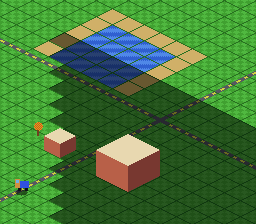
\includegraphics[width=0.75\textwidth]{figures/iso-shading-demo.png}
	\caption{Fog of War and a Vehicle Shadow}
	\label{fig:m2-shading-demo}
\end{figure}

\section{Layers, Priority and Height}
\label{sec:m2-layers}

Background 1 is in front of background 2. A pixel of background 1 whose value is not 0 hides the pixel of background 2
at the same screen position, and if both are 0 the device shows palette entry 0 (Section~\ref{sec:compositing}). The
disable bits \texttt{B1D} and \texttt{B2D} of the Base Configuration register make the corresponding background
transparent. The two backgrounds have their own tilemap, tile data, scroll and palette registers; they share nothing
but the palette. Background 4 is not drawn in Mode 2.

Because each background scrolls independently, the two can be positioned relative to each other by any amount. That is
what a height offset is: a background whose \texttt{SCRY} is $h$ smaller than another's is drawn $h$ pixels lower on
the screen, and one whose \texttt{SCRY} is larger is drawn higher. The scroll is not part of the tile data: a program
scrolls a layer freely and the whole picture moves with it. What matters is the offset between the two layers. The
tiles of a layer are cut along its own grid, and a layer with a different scroll has its grid in a different place on
the screen, so the tool that slices the artist's picture is told the scroll each layer is drawn at while the picture is
cut (Section~\ref{sec:m2-authoring}), and the program keeps the offset between the layers after that. Offset layers are
for one purpose: a tall object overhangs the cells behind it, and in one layer it must share those cells with whatever
else is there, so objects that would otherwise conflict are put on a layer with a different grid. Two layers cannot
make every overhang work. Anything that moves is a sprite, or the program rewrites tiles as it moves.

\section{Authoring Tiles}
\label{sec:m2-authoring}

An artist draws in screen space: a picture of diamonds, roads, water and buildings, as it should appear. A tool turns
that picture into tilemaps and tiles with this algorithm:

\begin{enumerate}
	\item Choose the scroll $(\texttt{SCRX}, \texttt{SCRY})$ at which the picture is drawn. It only decides where the picture
	      falls on the layer's grid; the program may scroll the layer anywhere afterwards. A layer that is to sit offset from
	      another has its own scroll here, and the program keeps that difference.
	\item For each pixel $(x, y)$ of the picture, find the texel $(u, v)$ shown by the plane pixel $(x + \texttt{SCRX},\, y +
		      \texttt{SCRY})$ and the cell and the position within the tile (Section~\ref{sec:m2-geometry}), and store the pixel's
	      value there.
	\item Texels that no pixel reaches stay 0, transparent.
	\item Give each different tile image a tile number, and reuse the number for identical images. Tile 0 is the empty tile.
	\item Pack each tile into the staircase layout and write the tilemap entry of each cell.
\end{enumerate}

Because the mapping is a bijection, the result shows the picture again pixel for pixel. A picture of ground, roads, a
lake and two buildings, drawn in screen space and sliced this way, is shown with no differing pixel.

The tiles of a picture drawn on a regular lattice repeat, and step 4 saves their storage: the ground of the example
picture, a 256 by 224 screen of grass, two roads and a lake, takes 15 tiles, counting the empty tile 0. The two
buildings of the example, whose walls overhang many cells, take 28, again counting the empty tile, and only because
they were drawn once and cut up by the tool. An artist does not need to draw cell by cell.

\section{Restrictions}
\label{sec:m2-restrictions}

Mode 2 has these restrictions, all of which are consequences of the design above:

\begin{itemize}
	\item Two isometric backgrounds and an orthogonal status layer. The status layer does not scroll, and its flip bits are
	      ignored.
	\item 16 by 16 texel tiles only. The tile size bits of the \texttt{TILESIZE} register are ignored. An 8 by 8 texel tile would be a 16 by 8
	      diamond; it is not supported.
	\item A tilemap of 32 or 64 cells across and down (Section~\ref{sec:tilemap-size}).
	\item Tiles cannot be flipped: the flip bits darken and lighten instead (Section~\ref{sec:m2-shading}). A mirrored tile is a
	      different tile, and the tool writes it.
	\item The priority bit is ignored.
	\item No fetch slots for sprites in the visible part of a line.
	\item 4 or 2 bits per texel, chosen for each isometric background (Section~\ref{sec:m2-two-bit}).
	\item No rotation of the view. Art is drawn for one facing, and a program that shows several facings keeps a set of tiles for
	      each.
	\item Heights are not part of the hardware. A raised terrain is a background with a different scroll
	      (Section~\ref{sec:m2-layers}).
\end{itemize}

\section{A Worked Example}
\label{sec:m2-example}

Figure~\ref{fig:m2-demo} shows the picture the device draws for an example scene. The ground, on background 2, is a map
of grass, two crossing roads, and a lake with a sandy shore. The buildings, on background 1, are a tower of two cells
by two and a house of one cell. Background 1 is scrolled down by 8 pixels, and its picture was sliced against the grid
that results; the picture on the screen is the same however it is sliced.

\begin{figure}[H]
	\centering
	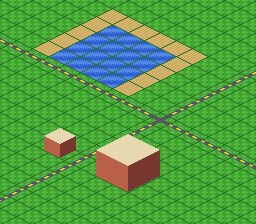
\includegraphics[width=0.75\textwidth]{figures/iso-demo.png}
	\caption{Mode 2 Output for the Example Scene}
	\label{fig:m2-demo}
\end{figure}

The registers were set as follows:

\begin{table}[H]
	\centering
	\begin{tabular}{lll}
		\toprule
		\textbf{Register}     & \textbf{Background 1 (buildings)}                       & \textbf{Background 2 (ground)}   \\
		\midrule
		\texttt{CONFIG}       & \multicolumn{2}{c}{\texttt{MODE} = 1, \texttt{B3D} = 1}                                    \\
		Tilemap address       & \texttt{0x8000}                                         & \texttt{0x8400}                  \\
		Tile data address     & \texttt{0x9000}                                         & \texttt{0xA000}                  \\
		Scroll X, scroll Y    & 0, 8                                                    & 0, 0                             \\
		Palette configuration & \texttt{OFFSET} 0x10, 16 colours                        & \texttt{OFFSET} 0x00, 16 colours \\
		Palette entries used  & 0x11--0x13                                              & 1--8                             \\
		\bottomrule
	\end{tabular}
	\caption{Register Values of the Example Scene}
	\label{tab:m2-example-regs}
\end{table}

\section{Programming Mode 2}

A program uses Mode 2 as follows:

\begin{enumerate}
	\item During vertical blanking, load the palette and write the tile data and the tilemaps into video memory.
	\item Write the tilemap and tile data address registers and the palette configuration registers of backgrounds 1 and 2.
	\item Write the Base Configuration register with \texttt{MODE} = 1.
	\item Each frame, during vertical blanking, write the scroll registers. The scrolls of the two backgrounds are independent.
\end{enumerate}

To leave Mode 2, write \texttt{MODE} = 0 during vertical blanking. The address and palette registers keep their values,
so Mode 1 can reuse them.

\chapter{Mode 3: Orthogonal Backgrounds over an Isometric One}
\label{ch:mode3}

\section{Overview}

Mode 3 keeps one isometric background and gives the fetch slots of the other to two orthogonal ones. It is for a game
with an isometric ground and a user interface that needs more than the status layer of Mode 2: a status display and a
layer of windows over it, with the map, and the vehicles and buildings as sprites, underneath.

\begin{description}
	\item[Selected by:] \texttt{MODE} = 2 in the Base Configuration register.
	\item[Layers:] Orthogonal backgrounds 1 and 2 in front, and an isometric background 3 behind them. The order front to back is
	      S1, B1, S2, B2, S3, B3, as in Mode 1 (Section~\ref{sec:m1-priority}).
	\item[Registers:] Each background uses its own tilemap, tile data, scroll and palette configuration registers, as in Mode 1.
	      Background 3 is the isometric one, so \texttt{B3MAP}, \texttt{B3TILES}, \texttt{B3SCRX}, \texttt{B3SCRY} and
	      \texttt{B3PAL} follow Mode 2 (Chapter~\ref{ch:mode2}).
\end{description}

Mode 3 adds no hardware to Mode 2. Each background is the same fetch unit as in the other modes, and the mode only says
which slots of a group of four pixels belong to which background. The price is the status layer of Mode 2: with no
spare slots there is no queue, and no second isometric background.

\section{The Orthogonal Backgrounds}

An orthogonal background is the background of Mode 1 (Chapter~\ref{ch:mode1}): a tilemap of 8 by 8 or 16 by 16 tiles,
32 by 32 entries or larger (Section~\ref{sec:tilemap-size}), that wraps in both directions. Its tilemap entry holds a
tile number and a palette selection (Section~\ref{sec:tilemap-entry}), and its flip bits and priority bit apply as they
do in Mode 1. Tiles are 4 bits per pixel, 16 words each (Section~\ref{sec:m1-tile-layout}), or, when \texttt{T2} is set
in its palette configuration register, 2 bits per pixel, 8 words each (Section~\ref{sec:flat-two-bit}). The palette is
chosen as in Section~\ref{sec:palette-select}, with the register's own \texttt{OFFSET}. Pixels of value 0 are
transparent. The priority bit puts a tile in front of every sprite layer.

\subsection{Scrolling}
\label{sec:m3-scrolling}

Each orthogonal background scrolls independently. Its scroll registers are sampled once per line, as in Mode 2. The
device fetches groups of four pixels aligned to the plane, so that group $g$ of the line is the plane group $\lfloor
	\texttt{SCRX}/4 \rfloor + g$. Plane group $q$ is the left half of tile column $\lfloor q/2 \rfloor \bmod 32$ when $q$
is even and the right half when it is odd, and the row is $(\text{line} + \texttt{SCRY}) \bmod 256$. When \texttt{SCRX}
is not a multiple of four, the line's first pixel is at position $\texttt{SCRX} \bmod 4$ in a window of two groups, as
in Section~\ref{sec:m2-fetch}. Fine scrolling costs no extra fetches.

\section{Fetch Schedule}

The eight slots of a group of four pixels have fixed owners:

\begin{table}[H]
	\centering
	\begin{tabular}{cp{5.8cm}p{5.2cm}}
		\toprule
		\textbf{Slot} & \textbf{Fetch}                                                & \textbf{Used}                            \\
		\midrule
		0             & Background 1 tilemap entry                                    & Always (2-bit tiles: every second group) \\
		1             & Background 1 tile data word                                   & Always (2-bit tiles: every second group) \\
		2, 3          & The same two fetches for background 2                         &                                          \\
		4--7          & The four fetches of an isometric background, for background 3 & As in Table~\ref{tab:m2-slots}           \\
		\bottomrule
	\end{tabular}
	\caption{Mode 3 Fetch Slots per Group of Four Pixels}
	\label{tab:m3-slots}
\end{table}

The orthogonal backgrounds use four slots in every group, and the isometric background uses two to four, so a group
uses six or more of the eight and the worst case uses all eight. No slot is left for anything else in the visible part
of a line. Sprites are fetched in the horizontal blanking interval, as in the other modes (Chapter~\ref{ch:sprites}),
and the back-porch prefetch of two groups is the same as in Mode 2.

Because no background depends on a slot that another leaves spare, the schedule is fixed and needs no queue.

\section{Differences from Mode 2}

\begin{itemize}
	\item There is no status layer: the orthogonal backgrounds take its place, and \texttt{B3D} disables the isometric
	      background.
	\item \texttt{B1D}, \texttt{B2D} and \texttt{B3D} disable the corresponding background, as in Mode 2.
	\item The isometric background is background 3, so it is behind the orthogonal ones. The shading bits of its tilemap entries
	      (Section~\ref{sec:m2-shading}) apply to it; the orthogonal backgrounds ignore the flip bits.
	\item Only one background is isometric, so the height offsets of Section~\ref{sec:m2-layers} between two isometric
	      backgrounds are not available. Buildings and vehicles are sprites.
\end{itemize}

\section{Restrictions}

\begin{itemize}
	\item One isometric background, with the restrictions of Mode 2 (Section~\ref{sec:m2-restrictions}).
\end{itemize}

\section{Programming Mode 3}

\begin{enumerate}
	\item Write the tilemap, tile data and palettes of the three backgrounds. The orthogonal tiles use the format of
	      Section~\ref{sec:m1-tile-layout} or~\ref{sec:flat-two-bit}; the isometric tiles use the staircase format
	      (Section~\ref{sec:m2-tile-format}) or its 2-bit form.
	\item Set \texttt{B1MAP}--\texttt{B3MAP}, \texttt{B1TILES}--\texttt{B3TILES} and the palette and scroll registers.
	\item Write 2 to the \texttt{MODE} field. Do it in vertical blanking: a change during a line takes effect at the start of the
	      next one.
\end{enumerate}

\chapter{Sprites}
\label{ch:sprites}

\section{Overview}

The device draws three layers of sprites, S1 to S3, each 4 bits per pixel. The sprites are described by a table of 128
entries of 32 bits each, mapped at offsets \texttt{0x7000}--\texttt{0x70FF} of the device segment, and their tile data
is at the address in the \texttt{STILES} register. A sprite layer sits between background layers in the front-to-back
order S1, B1, S2, B2, S3, B3. Sprite tiles are 8 by 8 or 16 by 16 pixels, chosen for each sprite layer by the
\texttt{TILESIZE} register.

\section{Sprite Table Entry}
\label{sec:sprite-entry}

Each entry is two words. The table is internal memory of the device: reading it costs no video memory bandwidth, which
is what lets the device scan all 128 entries while it draws the previous line. The contents of the table are undefined
at reset. A sprite whose layer field is 3 is hidden.

\begin{table}[H]
	\centering
	\begin{tabular}{llp{7.5cm}}
		\toprule
		\textbf{Word} & \textbf{Bits} & \textbf{Field}                                                           \\
		\midrule
		0             & 15            & \texttt{V}: flip vertically                                              \\
		0             & 14            & \texttt{H}: flip horizontally                                            \\
		0             & 13--11        & \texttt{P}: sprite palette 0--7                                          \\
		0             & 10--9         & \texttt{L}: sprite layer, 0--2 for S1--S3; 3 hides the sprite            \\
		0             & 8--0          & \texttt{X}: left edge, a signed 9-bit number ($-256$ to 255)             \\
		1             & 15--8         & \texttt{Y}: top line, 0--255, wrapping, so a sprite can enter from above \\
		1             & 7--0          & \texttt{T}: tile number                                                  \\
		\bottomrule
	\end{tabular}
	\caption{Sprite Table Entry}
	\label{tab:sprite-entry}
\end{table}

The tile number is 8 bits because the entry has no room for more: 32 bits cannot hold a 9-bit X, an 8-bit Y, three
flags, a 3-bit palette and a 2-bit layer together with a 10-bit tile number, as a background tilemap entry has. A sheet
of 256 tiles is 4,096 words of 8 by 8 sprites, or 16,384 words (half of video memory) of 16 by 16 sprites. A program
that needs more switches the \texttt{STILES} register between frames.

\section{Sprite Tile Data}

A sprite tile is stored as a background tile is (Sections~\ref{sec:m1-tile-layout} and~\ref{sec:flat-16}), 4 bits per
pixel, leftmost pixel in bits 15--12 of a word. An 8 by 8 tile is 16 words, two for each row. A 16 by 16 tile is four 8
by 8 quadrants in the order top left, top right, bottom left, bottom right, 64 words in all. The word for pixel column
$c$ and row $r$ of tile $t$ is at
\[
	\text{STILES} + t \cdot (s^2/4) + 16 q + 2 (r \bmod 8) + \lfloor (c \bmod 8)/4 \rfloor ,
\]
where $s$ is the sprite size and the quadrant $q$ is $0$ for an 8 by 8 tile and $2\lfloor r/8 \rfloor + \lfloor c/8
	\rfloor$ for a 16 by 16 one. A row of a 16 by 16 sprite is therefore two words from the left quadrant and two from the
right. Value 0 is transparent. A pixel of value $v$ in a sprite of palette $p$ selects palette entry $\texttt{0x80} +
	16p + v$, so the sprites own the upper half of the palette: eight palettes of 16 entries, which is independent of the
background palette offsets. The exception is value 15 of palette 7 when \texttt{SHD} is set, the shadow colour
(Section~\ref{sec:sprite-shadow}).

\section{Shadow Pixels}
\label{sec:sprite-shadow}

When the \texttt{SHD} bit of the Base Configuration register is set, a sprite pixel of value 15 in sprite palette 7 is
a shadow. With the bit clear, which it is at reset, it is an ordinary colour. A shadow draws nothing itself; it darkens
what is behind its sprite layer, as the shading of Section~\ref{sec:m2-shading} does (each colour channel halved). It
is for the shadow under a vehicle or a building. It works in every mode. While \texttt{SHD} is set, the palette entry
\texttt{0xFF} is never used.

The line buffer holds one sprite pixel per column, so the rules for shadows are simple: a shadow pixel never covers a
drawn sprite pixel, and a drawn sprite pixel always replaces a shadow pixel, whatever their layers. A shadow therefore
darkens the backgrounds, not other sprites, and darkening does not accumulate.

\section{Drawing a Line}
\label{sec:sprite-line}

The device draws sprites with a line buffer of 256 entries, which it fills before the line is shown:

\begin{enumerate}
	\item \textbf{Scan.} During the visible part of the previous line the device walks the table and keeps the first 32
	      sprites, in table order, whose rows cross the next line and whose layer is neither hidden nor disabled in the Base
	      Configuration register. A sprite is on the line when $(\text{line} - Y) \bmod 256$ is less than its size.
	      Further sprites on the line are dropped.
	\item \textbf{Fetch.} In the horizontal blanking interval it reads one row of tile data for each kept sprite, one
	      word per PPU cycle. A word with no pixel on the screen is not read.
	\item \textbf{Paint.} Each word is expanded into the line buffer. Where sprites overlap, the one on the lower layer
	      number wins, then the one with the lower table index. The buffer holds one pixel per column, with its palette
	      entry and its layer.
\end{enumerate}

Keeping only the frontmost sprite pixel is enough. A sprite pixel that lies behind another sprite pixel could never be
the one shown: whatever would cover it, the frontmost sprite pixel is in front of the same things.

When the line is shown, the compositor places the buffered sprite pixel among the backgrounds in the order S1, B1, S2,
B2, S3, B3 (and, in Mode 1, B3 last), taking the first opaque pixel. This is the same rule in both modes; Mode 2 simply
has no third background.

\section{How Many Sprites}
\label{sec:sprite-budget}

\subsection{Fetch Budget}

The horizontal blanking interval is 340 master clocks, 170 PPU cycles, and neither mode fetches background data in it
except for a prefetch of 22 cycles before the first pixel (16 for the two isometric backgrounds, six for the status
layer). That leaves 148 video memory reads per line for sprites, whatever the mode. A sprite costs one read per word of
its row.

\begin{table}[H]
	\centering
	\begin{tabular}{rrrr}
		\toprule
		\textbf{Size} & \textbf{Reads per sprite} & \textbf{Fit in 148 reads} & \textbf{Reads for 32 sprites} \\
		\midrule
		8 by 8        & 2                         & 74                        & 64                            \\
		16 by 16      & 4                         & 37                        & 128                           \\
		\bottomrule
	\end{tabular}
	\caption{Sprite Fetch Cost per Line, Blanking Only}
	\label{tab:sprite-budget}
\end{table}

The time budget is therefore not the limit; 32 sprites of either size fit with room to spare. The limit is the capacity
of the line registers that hold a kept sprite between the scan and the fetch. The device keeps 32, and one sprite is
about 40 bits of state, so 32 is some 160 bytes of registers. A program can use all 128 entries in a frame, but no more
than 32 on any one line; a line that has more drops the highest-numbered ones, and sets the \texttt{SOV} bit of the
Status register (Chapter~\ref{ch:registers}).

\subsection{Using the Visible Slots as Well}

The fetch slots of the visible part of the line could be used as well, but the sprites for the next line could then no
longer be painted into the buffer that is being shown, so a second line buffer (another 256 entries) is needed.

\begin{description}
	\item[Mode 1] has one slot in each group of four pixels reserved for sprite tile data, 64 reads per line, taking the budget
	      to 218 reads: 109 sprites of 8 by 8, 54 of 16 by 16.
	\item[Mode 2] has no slot reserved, but some of its slots are spare. Which ones depends only on the scroll position, not on
	      the tile data (Section~\ref{sec:m2-spare-slots}), so the device can know in advance. Over all scroll positions 192 to
	      224 slots per line out of 512 are spare, 208 on average, and the status layer takes some of them.
\end{description}

Neither is needed to reach the line limit, so the device does not use them.

\section{Sprites in Modes 2 and 3}

Sprites are drawn the same way in Modes 2 and 3, at screen positions. In Mode 2, which has two isometric backgrounds,
the three sprite layers sit as S1, B1, S2, B2, S3. In Mode 3 the order is the same as in Mode 1, S1, B1, S2, B2, S3,
B3, with the isometric background last. A program sorts its sprites against the map itself: a lorry that is to pass
behind a tower on B1 goes on S2, one that is to pass in front goes on S1, and it changes layer as it crosses.
Figure~\ref{fig:sprite-demo} shows both: the lorry on S1 is in front of the tower, and the one on S2 would be hidden by
it.

\begin{figure}[H]
	\centering
	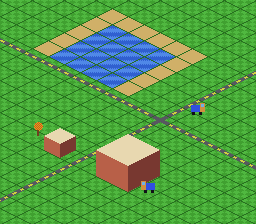
\includegraphics[width=0.75\textwidth]{figures/iso-sprite-demo.png}
	\caption{Two Lorries and a Tree over the Mode 2 Demonstration Scene}
	\label{fig:sprite-demo}
\end{figure}

\section{Programming Sprites}

\begin{enumerate}
	\item Write the sprite tile data into video memory, at the address that will be written to \texttt{STILES}.
	\item Write \texttt{STILES}, and the sprite tile size bits of the \texttt{TILESIZE} register.
	\item Write the table: entry $n$ is the words at offsets \texttt{0x7000} $+ 2n$ and \texttt{0x7001} $+ 2n$. Set the layer
	      field of every unused entry to 3.
	\item Make sure the sprite layers in use are not disabled in the Base Configuration register.
	\item Each frame, during vertical blanking, rewrite the \texttt{X} and \texttt{Y} fields of the sprites that moved.
\end{enumerate}

\section{Notes}

\begin{itemize}
	\item Scanning the 128 entries needs one read of the table per entry, at most 128 of the 512 PPU cycles of a line, from
	      internal memory.
	\item Sprites are not clipped to a window, and there is no priority bit per sprite beyond the layer.
\end{itemize}

\chapter{Timing}
\label{ch:timing}

\section{Clocks}

The device runs from the system's master clock. It does one PPU cycle every two master clocks, and one pixel every two
PPU cycles, which is four master clocks. Table~\ref{tab:clocks} gives the rates for the master clock of the SIRCUS
system, 21,477,272~Hz, which is the NTSC colour subcarrier frequency multiplied by six.

\begin{table}[H]
	\centering
	\begin{tabular}{lrr}
		\toprule
		\textbf{Clock} & \textbf{Master clocks} & \textbf{At 21,477,272 Hz} \\
		\midrule
		Master clock   & 1                      & 21,477,272 Hz             \\
		PPU cycle      & 2                      & 10,738,636 Hz             \\
		Pixel          & 4                      & 5,369,318 Hz              \\
		Line           & 1364                   & 15,746 Hz                 \\
		Frame          & 357,368                & 60.1 Hz                   \\
		\bottomrule
	\end{tabular}
	\caption{Clock Rates}
	\label{tab:clocks}
\end{table}

\section{The CPU Clock}
\label{sec:cpu-clock}

The CPU advances one execution phase on each rising edge of \texttt{CLKI} (\hwmanual{}). The system supplies the CPU
and the video device with the same \texttt{CLKI}, which is the only clock the device has, and \texttt{CLKI} is one PPU
cycle: the master clock divided by two, 10,738,636~Hz at 21,477,272~Hz. The figures that follow are consequences:

\begin{itemize}
	\item An ordinary instruction takes 6 \texttt{CLKI} cycles, 12 master clocks, so the CPU can run about 1.79 million
	      instructions a second.
	\item A line is 682 \texttt{CLKI} cycles, about 113 instructions, and a frame is 178,684 cycles. NTSC vertical blanking, 38
	      lines, is 25,916 cycles, about 4,300 instructions.
	\item The registers are sampled 228 master clocks, 114 cycles, after the start of a line. A line-compare interrupt is
	      recognised at an instruction boundary, so the handler's first instruction is fetched at best 6 and at worst about 12
	      cycles later (\archmanual{}, interrupt latency; more after a coprocessor call or a DMA transfer). That leaves about 100
	      cycles, some 16 instructions, for a handler to change a register before it takes effect on the same line.
	\item A \texttt{DMAT} of 255 words takes 522 cycles, three quarters of a line, and cannot be interrupted.
\end{itemize}

The video device never waits for the CPU, and it gives the CPU no wait states: every access to the device completes in
the cycle it is made (Section~\ref{sec:memory-vram-access}).

\section{Line Timing}

A line is 1364 master clocks, 682 PPU cycles, in three parts. A line begins with the horizontal sync pulse
(Section~\ref{sec:video-output}), and the picture follows the back porch; the front porch ends the line. The line
timing is fixed and the same in both modes:

\begin{table}[H]
	\centering
	\begin{tabular}{lrrl}
		\toprule
		\textbf{Part}       & \textbf{Master clocks} & \textbf{PPU cycles} & \textbf{Purpose}                    \\
		\midrule
		Sync and back porch & 260                    & 130                 & Nothing is drawn; Mode 2 prefetches \\
		Visible             & 1024                   & 512                 & 256 pixels at 4 master clocks each  \\
		Front porch         & 80                     & 40                  & Nothing is drawn                    \\
		\midrule
		\textbf{Line}       & \textbf{1364}          & \textbf{682}        &                                     \\
		\bottomrule
	\end{tabular}
	\caption{Line Timing}
	\label{tab:line-timing}
\end{table}

The visible time of a line is a whole number of master clocks per pixel: four.

\begin{figure}[H]
	\centering
	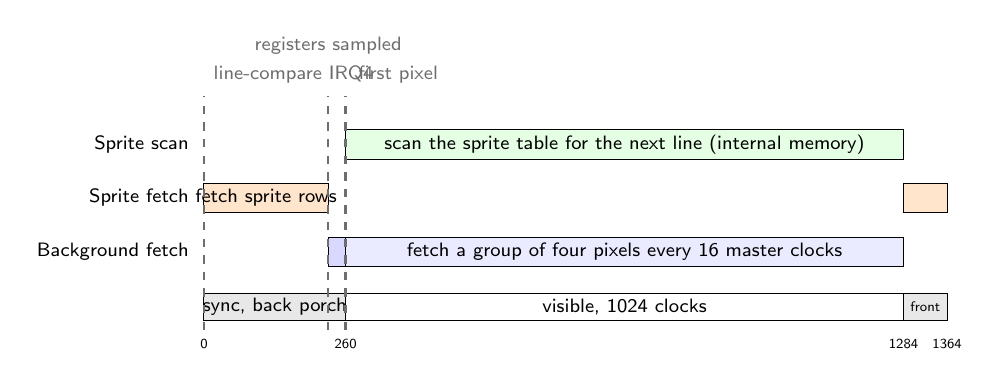
\begin{tikzpicture}[
			x=0.0057\textwidth,
			y=0.62cm,
			bar/.style={draw, minimum height=0.55cm, font=\scriptsize, align=center, inner sep=1pt},
			lane/.style={font=\scriptsize, anchor=east},
			marker/.style={dashed, thick, sircgray},
			note/.style={font=\scriptsize, text=sircgray}
		]
		% Line parts (1364 master clocks)
		\fill[sirclightgray] (0,0) rectangle (26,0.55);
		\fill[white] (26,0) rectangle (128.4,0.55);
		\fill[sirclightgray] (128.4,0) rectangle (136.4,0.55);
		\draw (0,0) rectangle (136.4,0.55);
		\draw (26,0) -- (26,0.55);
		\draw (128.4,0) -- (128.4,0.55);
		\node[font=\scriptsize] at (13,0.28) {sync, back porch};
		\node[font=\scriptsize] at (77.2,0.28) {visible, 1024 clocks};
		\node[font=\tiny] at (132.4,0.28) {front};
		% Lanes
		\node[lane] at (-1,1.4) {Background fetch};
		\draw[fill=blue!15] (22.8,1.1) rectangle (26,1.7);
		\draw[fill=blue!8] (26,1.1) rectangle (128.4,1.7);
		\node[font=\scriptsize] at (77.2,1.4) {fetch a group of four pixels every 16 master clocks};
		\node[lane] at (-1,2.5) {Sprite fetch};
		\draw[fill=orange!20] (0,2.2) rectangle (22.8,2.8);
		\draw[fill=orange!20] (128.4,2.2) rectangle (136.4,2.8);
		\node[font=\scriptsize] at (11.4,2.5) {fetch sprite rows};
		\node[lane] at (-1,3.6) {Sprite scan};
		\draw[fill=green!10] (26,3.3) rectangle (128.4,3.9);
		\node[font=\scriptsize] at (77.2,3.6) {scan the sprite table for the next line (internal memory)};
		% Markers
		\draw[marker] (0,-0.2) -- (0,4.6);
		\draw[marker] (22.8,-0.2) -- (22.8,4.6);
		\draw[marker] (26,-0.2) -- (26,4.6);
		\node[note, anchor=south west] at (0,4.65) {line-compare IRQ4};
		\node[note, anchor=south] at (22.8,5.25) {registers sampled};
		\node[note, anchor=south west] at (26.6,4.65) {first pixel};
		% Axis
		\foreach \x/\l in {0/0, 26/260, 128.4/1284, 136.4/1364} { \node[font=\tiny, anchor=north] at (\x,-0.2) {\l}; }
	\end{tikzpicture}
	\caption{Timeline of One Visible Line, in Master Clocks}
	\label{fig:line-timeline}
\end{figure}

\section{Frame Timing}

A frame is 262 lines on NTSC and 312 on PAL. Lines 0 to 223 are visible and draw the picture. The remaining lines, 38
on NTSC and 88 on PAL, are the vertical blanking interval, in which nothing is drawn and the CPU may update video
memory (Section~\ref{sec:memory-vram-access}). The device fetches nothing in these lines.

Table~\ref{tab:times} gives the times. They follow from the clocks: on NTSC the PPU cycle is 93.1~ns and a pixel, four
master clocks, is 186.2~ns.

\begin{table}[H]
	\centering
	\begin{tabular}{lrr}
		\toprule
		                       & \textbf{NTSC} & \textbf{PAL} \\
		\midrule
		Master clock           & 21.477~MHz    & 21.281~MHz   \\
		Line                   & 63.5~$\mu$s   & 64.1~$\mu$s  \\
		Frame                  & 16.64~ms      & 20.00~ms     \\
		Frame rate             & 60.10~Hz      & 50.00~Hz     \\
		Vertical blanking      & 2.41~ms       & 5.64~ms      \\
		Pixel                  & 186.2~ns      & 188.0~ns     \\
		Visible part of a line & 47.7~$\mu$s   & 48.1~$\mu$s  \\
		\bottomrule
	\end{tabular}
	\caption{Video Timing}
	\label{tab:times}
\end{table}

\subsection{PAL}

The \texttt{OUT} bit of the Status register says which the device is. PAL has the same picture, 256 by 224 pixels in
lines 0 to 223, at the top, and the same line timing of 1364 master clocks, but 312 lines per frame, so the vertical
blanking interval is longer. A program written for NTSC runs unchanged on PAL, with more time in vertical blanking and
a lower frame rate. With a PAL master clock of 21,281,370 Hz (the PAL colour subcarrier multiplied by 4.8) a frame is
425,568 master clocks, 50.0 Hz. The region is fixed when the device is made and is read from \texttt{OUT}.

\section{Interrupts}
\label{sec:interrupts}

The device has two interrupt sources, on different lines, so a handler knows which it is serving. The device races the
beam: it never waits for the CPU, so an interrupt is raised at a fixed point of the frame whether or not the CPU is
ready, and the time the CPU takes to respond is the program's concern. A program that shares \activelow{IRQ4} with
another device can read the \texttt{LIP} bit of the Status register to see whether the device's interrupt is the one
pending.

\subsection{Vertical Sync}

The vertical sync interrupt is the non-maskable interrupt, \activelow{NMI}, Level 5. It is edge-triggered, so the
device needs no acknowledgement: when \texttt{VIE} is set in the Interrupt Control register
(Section~\ref{sec:reg-intctl}), the device asserts the \activelow{NMI} pin for one PPU cycle at the first cycle of line
224, the start of vertical blanking. The program has the whole of vertical blanking to update video memory
(Section~\ref{sec:memory-vram-access}). The pulse is exactly one \texttt{CLKI} cycle (Section~\ref{sec:cpu-clock}). The
CPU samples \activelow{NMI} on every rising edge of \texttt{CLKI} except during reset (\hwmanual{}), so it does not
miss the pulse. A pulse that arrives while the handler of the previous one is still running, or while a Level 5 request
is pending, is not taken as an interrupt: it raises the Level Five Hardware Exception Conflict fault (\archmanual{}).
The handler must therefore return before the next vertical sync, 16.6~ms later on NTSC and 20.0~ms on PAL.

The \activelow{NMI} cannot be masked, so a program must install its handler before it sets \texttt{VIE}. A DMA transfer
cannot be interrupted, the \activelow{NMI} included. The edge is latched and the interrupt is taken when the transfer
ends, so it is delayed, not lost, but a transfer that spans line 224 shortens the time the program has in vertical
blanking by the delay. A program keeps its transfers short (Section~\ref{sec:cpu-clock} gives their lengths), or
arranges for them to finish before line 224.

\subsection{Line Compare}
\label{sec:line-interrupt}

The line-compare interrupt is interrupt level 4, \activelow{IRQ4}, the highest of the maskable levels. When
\texttt{LIE} is set, the device asserts the line at the first cycle of the line whose number is in the \texttt{LINE}
register (Section~\ref{sec:reg-line}). It fires on any line of the frame, visible or not, so lines 0 to 223 can be used
for raster effects. The \activelow{IRQ4} line is level-sensitive, so the device holds it asserted until the program
acknowledges it by writing any value to \texttt{LINE}, which also sets the line for the next interrupt, or by clearing
\texttt{LIE}. The \texttt{LIP} bit of the Status register is set while the interrupt is pending. A \texttt{LINE} value
at or beyond the number of lines in the frame never matches. If the line is reached again while an interrupt is still
pending, nothing is queued: the line is already asserted.

The palette is writable at any time and a write changes the pixels drawn after it; the registers are sampled once per
line, 32 master clocks before the first visible pixel in Mode 2 and Mode 3, so a register written within the 228 master
clocks after the interrupt takes effect on that line, and later ones on the next. The device does not wait for the CPU,
so how soon after the interrupt the CPU's write arrives is the program's concern, and a handler for a raster effect
must be short and of known length.

\section{Fetch Budget}

Reading video memory is the device's limit: one read per PPU cycle, eight per group of four pixels. The modes spend the
eight slots differently.

\begin{table}[H]
	\centering
	\begin{tabular}{lccc}
		\toprule
		\textbf{Use of the slots}                             & \textbf{Mode 1} & \textbf{Mode 2}    & \textbf{Mode 3}   \\
		\midrule
		Background tilemap entries                            & 4               & 2--4               & 3--4              \\
		Background tile data words                            & 4               & 2--4               & 3--4              \\
		Sprites                                               & 0               & 0                  & 0                 \\
		\midrule
		\textbf{Total, typical (Mode 2, 3) or fixed (Mode 1)} & \textbf{8}      & \textbf{4.75 of 8} & \textbf{6.4 of 8} \\
		\textbf{Total, worst case}                            & \textbf{8}      & \textbf{8}         & \textbf{8}        \\
		\bottomrule
	\end{tabular}
	\caption{Fetch Slots per Group of Four Pixels}
	\label{tab:fetch-budget}
\end{table}

\begin{figure}[H]
	\centering
	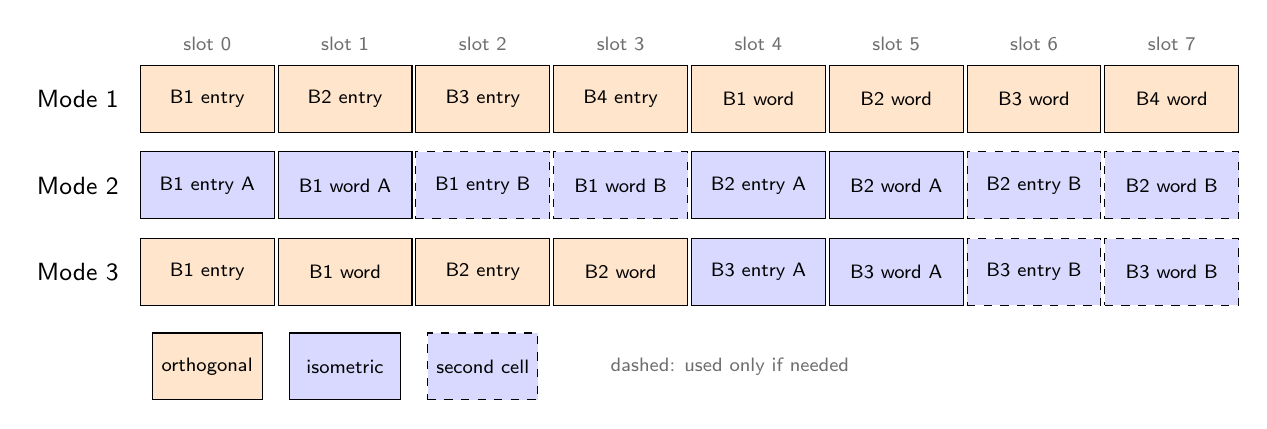
\begin{tikzpicture}[
			cell/.style={draw, minimum width=1.7cm, minimum height=0.85cm, font=\scriptsize, align=center, inner sep=1pt},
			flatc/.style={cell, fill=orange!20},
			isoc/.style={cell, fill=blue!15},
			isob/.style={cell, fill=blue!15, dashed},
			free/.style={cell, fill=gray!8, dashed},
			rowlab/.style={font=\small, anchor=east},
			head/.style={font=\scriptsize, text=sircgray}
		]
		\foreach \i in {0,...,7} { \node[head] at (\i*1.75,0.7) {slot \i}; }
		\node[rowlab] at (-1.0,0) {Mode 1};
		\foreach \i/\t in {0/B1 entry,1/B2 entry,2/B3 entry,3/B4 entry,4/B1 word,5/B2 word,6/B3 word,7/B4 word} { \node[flatc] at (\i*1.75,0) {\t}; }
		\node[rowlab] at (-1.0,-1.1) {Mode 2};
		\foreach \i/\t in {0/B1 entry A,1/B1 word A,4/B2 entry A,5/B2 word A} { \node[isoc] at (\i*1.75,-1.1) {\t}; }
		\foreach \i/\t in {2/B1 entry B,3/B1 word B,6/B2 entry B,7/B2 word B} { \node[isob] at (\i*1.75,-1.1) {\t}; }
		\node[rowlab] at (-1.0,-2.2) {Mode 3};
		\foreach \i/\t in {0/B1 entry,1/B1 word,2/B2 entry,3/B2 word} { \node[flatc] at (\i*1.75,-2.2) {\t}; }
		\foreach \i/\t in {4/B3 entry A,5/B3 word A} { \node[isoc] at (\i*1.75,-2.2) {\t}; }
		\foreach \i/\t in {6/B3 entry B,7/B3 word B} { \node[isob] at (\i*1.75,-2.2) {\t}; }
		% Legend
		\node[flatc, minimum width=1.4cm] at (0,-3.4) {orthogonal};
		\node[isoc, minimum width=1.4cm] at (1.75,-3.4) {isometric};
		\node[isob, minimum width=1.4cm] at (3.5,-3.4) {second cell};
		\node[head, anchor=west] at (5.0,-3.4) {dashed: used only if needed};
	\end{tikzpicture}
	\caption{Who Uses Each Fetch Slot of a Group of Four Pixels}
	\label{fig:slot-map}
\end{figure}

The status layer of Mode 2 takes its reads from the slots the isometric backgrounds leave spare, through a queue
(Section~\ref{sec:m2-status-layer}); they are not in the table. Mode 3's orthogonal backgrounds read a tilemap entry
and a tile word in every group, at fixed slots (Chapter~\ref{ch:mode3}); with 2-bit tiles they read only in every
second group. A mode with more backgrounds or a different mix of fetches than these needs more reads per group, such a
queue, or a faster memory.

\section{Pixel Pipeline}

The device draws a group of four pixels in two stages. During one group the device fetches the data for a later group
and, at the start of the group, combines the data it already has into four finished pixels, which are shown one at a
time over the group. Mode 1 combines the fetches of the previous group; Mode 2 combines the data it prefetched
(Section~\ref{sec:m2-fetch}). The first pixels of a line in Mode 1 are at the position the scroll registers give
(Section~\ref{sec:m1-scrolling}).

Figure~\ref{fig:fetch-timing} shows the schedule of one group in Modes 1 and 3, one read to a \texttt{CLKI} cycle, with
the four pixels that are shown while it is made. A pixel lasts two cycles. In Mode 3 the reads of the second cell of
the isometric background are made only when the group straddles two cells.

\begin{figure}[H]
	\centering
	\small
	\begin{tikztimingtable}[sirc timing diagram]
		CLKI                  & L 7{0.5H 0.5L}                                                  \\
		Slot                  & D{0} D{1} D{2} D{3} D{4} D{5} D{6} D{7}                         \\
		Mode 1 read           & D{B1e} D{B2e} D{B3e} D{B4e} D{B1w} D{B2w} D{B3w} D{B4w}         \\
		Mode 3 read           & D{B1e} D{B1w} D{B2e} D{B2w} D{B3e} D{B3w} D{B3e'} D{B3w'}       \\
		Pixel shown           & 2D{p0} 2D{p1} 2D{p2} 2D{p3}                                     \\
	\end{tikztimingtable}
	\caption{Fetch Schedule of One Group of Four Pixels (e: Tilemap Entry, w: Tile Word, $'$: Second Cell)}
	\label{fig:fetch-timing}
\end{figure}

\chapter{Signal Timing}
\label{ch:signal-timing}

This chapter gives the timing of the pins of the device (Chapter~\ref{ch:package}): the bus cycles in which the CPU
reads and writes it, the interrupt outputs, reset, and the video output. Chapter~\ref{ch:timing} gives the timing
inside the device, in the same units.

\section{Reading the Figures}

The figures follow the conventions of the bus timing diagrams of the \hwmanual{}. Each labeled interval is one
\texttt{CLKI} cycle, which is one PPU cycle, seen between rising edges. Waveform rows show physical levels: for an
active-low signal, \texttt{L} means asserted. Bands show a value; an empty band carries no defined value, and a
three-state signal that is not driven is drawn as a flat line at mid-level. The pulses in the \texttt{Sample} row mark
the rising edges at which the device samples the bus. Electrical delays are not specified, so the figures show logical
timing only.

\section{Bus Cycles}
\label{sec:signal-bus}

The device answers every cycle in which \activelow{CS} and \activelow{BAS} are both asserted, and it answers in the
cycle itself: \activelow{BACK} is asserted from the start of the cycle, so the CPU accepts the cycle at the next rising
edge and never waits (Chapter~\ref{ch:package}).

\subsection{Writes}

The CPU presents the offset on A0--A15, the data on D0--D15 and BRW low, just after the rising edge that starts the
cycle. The device takes the data at the rising edge that ends the cycle; the register, palette entry, video memory word
or sprite table word holds the new value from that edge, and a read in the next cycle returns it. A write to an offset
that is not stored, or one that the rules of Section~\ref{sec:memory-vram-access} discard, is acknowledged in the same
way.

\begin{figure}[H]
	\centering
	\small
	\begin{tikztimingtable}[sirc timing diagram]
		CLKI             & L 2{0.5H 0.5L}              \\
		Phase            & D{access} D{next} D{}       \\
		\activelow{CS}   & L H H                       \\
		\activelow{BAS}  & L H H                       \\
		BRW              & L H H                       \\
		A0--A15          & D{offset} D{} D{}           \\
		D0--D15          & D{data} Z Z                 \\
		\activelow{BACK} & L H H                       \\
		Stored word      & D{old} 2D{new}              \\
		Sample           & 0.95L 0.1H 1.95L            \\
	\end{tikztimingtable}
	\caption{Write Cycle}
	\label{fig:signal-write}
\end{figure}

\subsection{Reads}

On a read the device drives D0--D15 with the word the offset selects, from the start of the cycle to its end, and
releases the bus after it. The word is valid before the rising edge that ends the cycle, which is the edge at which the
CPU samples it. A read changes nothing in the device; no register has a side effect on a read.

\begin{figure}[H]
	\centering
	\small
	\begin{tikztimingtable}[sirc timing diagram]
		CLKI             & L 2{0.5H 0.5L}              \\
		Phase            & D{access} D{next} D{}       \\
		\activelow{CS}   & L H H                       \\
		\activelow{BAS}  & L H H                       \\
		BRW              & H H H                       \\
		A0--A15          & D{offset} D{} D{}           \\
		D0--D15          & D{data} Z Z                 \\
		\activelow{BACK} & L H H                       \\
		Sample           & 0.95L 0.1H 1.95L            \\
	\end{tikztimingtable}
	\caption{Read Cycle}
	\label{fig:signal-read}
\end{figure}

\subsection{Consecutive Cycles}

The device accepts one access in every cycle, with no recovery time between accesses. A DMA transfer, which makes one
bus cycle for each word (\hwmanual{}), therefore moves one word per \texttt{CLKI} cycle into the palette, the sprite
table or video memory, whichever the offsets address.

\begin{figure}[H]
	\centering
	\small
	\begin{tikztimingtable}[sirc timing diagram]
		CLKI             & L 5{0.5H 0.5L}                                        \\
		Phase            & D{Setup} D{Write 1} D{Write 2} D{Write 3} D{} D{}     \\
		\activelow{CS}   & H L L L H H                                           \\
		\activelow{BAS}  & H L L L H H                                           \\
		BRW              & H L L L H H                                           \\
		A0--A15          & D{} D{v} D{v+1} D{v+2} D{} D{}                        \\
		D0--D15          & Z D{d0} D{d1} D{d2} Z Z                               \\
		\activelow{BACK} & H L L L H H                                           \\
		Last word stored & 2D{} D{v} D{v+1} 2D{v+2}                              \\
		Sample           & 1.95L 0.1H 0.9L 0.1H 0.9L 0.1H 1.95L                  \\
	\end{tikztimingtable}
	\caption{Three-Word DMA Write into the Device}
	\label{fig:signal-dma}
\end{figure}

\subsection{The Start of Vertical Blanking}
\label{sec:signal-vblank}

Video memory and the sprite table are open to the CPU from the first cycle of line 224 to the last cycle of line 261,
and at any time while \texttt{GD} is set (Section~\ref{sec:memory-vram-access}). The gate changes at a line boundary,
so it is exact to the cycle. A write in the last cycle of line 223 is discarded; a write in the first cycle of line 224
is stored. The vertical sync interrupt is raised in that same first cycle (Section~\ref{sec:interrupts}), and the CPU
takes it at the end of the instruction in progress, so the handler's first access to video memory is some cycles later
than the figure shows.

\begin{figure}[H]
	\centering
	\small
	\begin{tikztimingtable}[sirc timing diagram]
		CLKI              & L 3{0.5H 0.5L}                     \\
		Line              & D{223} D{223} D{224} D{224}        \\
		Cycle in line     & D{680} D{681} D{0} D{1}            \\
		\activelow{CS}    & L L L L                            \\
		\activelow{BAS}   & L L L L                            \\
		BRW               & L L L L                            \\
		A0--A15           & D{v} D{v+1} D{v+2} D{v+3}          \\
		D0--D15           & D{d0} D{d1} D{d2} D{d3}            \\
		\activelow{BACK}  & L L L L                            \\
		Video memory open & L L H H                            \\
		Word stored       & D{no} D{no} D{yes} D{yes}          \\
		\activelow{NMI}   & H H L H                            \\
	\end{tikztimingtable}
	\caption{Video Memory Writes across the Start of Vertical Blanking (\texttt{VIE} set)}
	\label{fig:signal-vblank}
\end{figure}

\section{Interrupt Timing}
\label{sec:signal-interrupts}

The interrupt outputs change just after a rising edge of \texttt{CLKI}, like the other outputs of the device. The CPU
samples them at the rising edge that ends the cycle.

\subsection{Vertical Sync}

Figure~\ref{fig:signal-vblank} shows the pulse: \activelow{NMI} is asserted for the whole of the first cycle of line
224 and deasserted in the next, when \texttt{VIE} is set in the Interrupt Control register. The pulse is one
\texttt{CLKI} cycle, which the CPU always samples, and the device does not wait for or expect an acknowledgement
(Section~\ref{sec:interrupts}).

\subsection{Line Compare}

\activelow{IRQ4} is asserted at the first cycle of the line whose number is in \texttt{LINE}, when \texttt{LIE} is set,
and is held. It is released by the program, with a write to \texttt{LINE}, or by clearing \texttt{LIE}.
The \texttt{LIP} bit of the Status register follows the output.

\begin{figure}[H]
	\centering
	\small
	\begin{tikztimingtable}[sirc timing diagram]
		CLKI              & L 3{0.5H 0.5L}                     \\
		Line              & D{N-1} D{N-1} D{N} D{N}            \\
		Cycle in line     & D{680} D{681} D{0} D{1}            \\
		\texttt{LINE}     & 4D{N}                              \\
		\texttt{LIE}      & 4H                                 \\
		\activelow{IRQ4}  & H H L L                            \\
		\texttt{LIP}      & L L H H                            \\
	\end{tikztimingtable}
	\caption{Line-Compare Interrupt Raised at the Start of Line N}
	\label{fig:signal-irq-raise}
\end{figure}

The acknowledging write is an ordinary write cycle. The device releases \activelow{IRQ4} and clears \texttt{LIP} at the
rising edge that ends the write, so the line is high in the cycle after it. A program should write \texttt{LINE} early
in its handler, and before it returns, because \activelow{IRQ4} is level-sensitive and the CPU recognises the interrupt
again if the line is still asserted when the handler ends (Section~\ref{sec:interrupts}).

\begin{figure}[H]
	\centering
	\small
	\begin{tikztimingtable}[sirc timing diagram]
		CLKI              & L 3{0.5H 0.5L}                     \\
		Phase             & D{access} D{next} D{} D{}          \\
		\activelow{CS}    & L H H H                            \\
		\activelow{BAS}   & L H H H                            \\
		BRW               & L H H H                            \\
		A0--A15           & D{0x0015} D{} D{} D{}              \\
		D0--D15           & D{line} Z Z Z                      \\
		\activelow{BACK}  & L H H H                            \\
		\texttt{LINE}     & D{old} 3D{line}                    \\
		\activelow{IRQ4}  & L H H H                            \\
		\texttt{LIP}      & H L L L                            \\
		Sample            & 0.95L 0.1H 2.95L                   \\
	\end{tikztimingtable}
	\caption{Acknowledging the Line-Compare Interrupt with a Write to \texttt{LINE}}
	\label{fig:signal-irq-ack}
\end{figure}

\section{Reset}
\label{sec:signal-reset}

\activelow{RST} is sampled at each rising edge of \texttt{CLKI}. Every register takes its reset value at the first edge
at which \activelow{RST} is sampled asserted (Table~\ref{tab:reset}), and the outputs go to their idle state: the
interrupt outputs are deasserted, \activelow{CSYNC} is high, and the colour outputs are at black. The line and cycle
counters are held at the first cycle of line 0 while \activelow{RST} is asserted. The first cycle of line 0 is the cycle
that follows the rising edge at which \activelow{RST} is first sampled deasserted. The contents of the palette, video
memory and sprite table are undefined after reset (Chapter~\ref{ch:registers}).

\begin{figure}[H]
	\centering
	\small
	\begin{tikztimingtable}[sirc timing diagram, timing/xunit=3em]
		CLKI              & L 9{0.5H 0.5L}                                   \\
		\activelow{RST}   & 6L 4H                                            \\
		Registers         & D{any} 9D{reset values}                          \\
		Line and cycle    & D{} 6D{held at line 0, cycle 0} D{0} D{1} D{2}   \\
		Interrupts        & 10H                                           \\
		\activelow{CSYNC} & 7H 3L                                            \\
		R, G, B           & 10D{black}                                       \\
	\end{tikztimingtable}
	\caption{Reset, with \activelow{RST} Held for the Minimum of Six Cycles}
	\label{fig:signal-reset}
\end{figure}

\section{Video Output}
\label{sec:video-output}

The video outputs follow the line timing of Chapter~\ref{ch:timing}. A new pixel appears on R, G and B every four
master clocks, at the pixel boundary, and the colour outputs are at black outside the visible part of the line, in the
vertical blanking interval, and in forced blank. The brightness setting scales the colour before conversion
(Section~\ref{sec:reg-base-config}).

\subsection{Horizontal Sync}

\activelow{CSYNC} is asserted for the first 100 master clocks (50 cycles) of every line, and is high for the remaining 1264.
The pulse begins at the first cycle of the line, the same cycle at which the line-compare interrupt is raised. The back
porch follows it, and the first pixel is 160 master clocks after the end of the pulse. The line ends with the front
porch, 80 master clocks; the 64 clocks before the first pixel and the 44 before the front porch are black, so the picture
has a narrow black border on each side.

\begin{figure}[H]
	\centering
	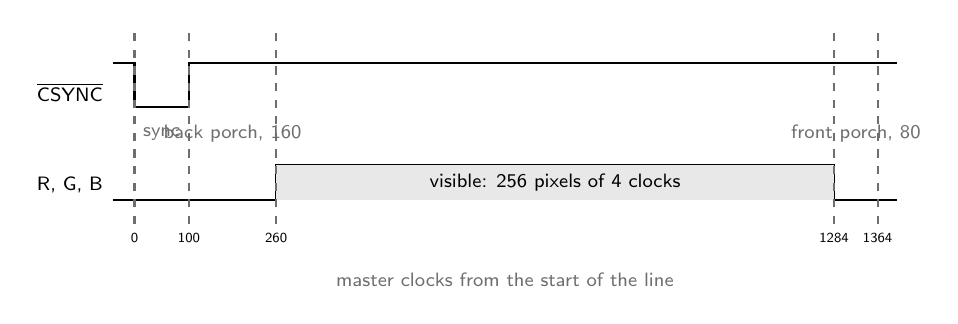
\begin{tikzpicture}[
			x=0.0057\textwidth,
			y=0.62cm,
			lane/.style={font=\scriptsize, anchor=east},
			marker/.style={dashed, thick, sircgray},
			note/.style={font=\scriptsize, text=sircgray}
		]
		% x is in units of 10 master clocks
		\node[lane] at (-4,3.3) {\activelow{CSYNC}};
		\draw[thick] (-4,3.9) -- (0,3.9) -- (0,3.0) -- (10,3.0) -- (10,3.9) -- (140,3.9);
		\node[lane] at (-4,1.4) {R, G, B};
		\draw[thick] (-4,1.1) -- (26,1.1) -- (26,1.8) -- (128.4,1.8) -- (128.4,1.1) -- (140,1.1);
		\fill[sirclightgray] (26,1.1) rectangle (128.4,1.8);
		\node[font=\scriptsize] at (77.2,1.45) {visible: 256 pixels of 4 clocks};
		\node[note] at (5,2.45) {sync};
		\node[note] at (18,2.45) {back porch, 160};
		\node[note] at (132.4,2.45) {front porch, 80};
		\draw[marker] (0,0.6) -- (0,4.6);
		\draw[marker] (10,0.6) -- (10,4.6);
		\draw[marker] (26,0.6) -- (26,4.6);
		\draw[marker] (128.4,0.6) -- (128.4,4.6);
		\draw[marker] (136.4,0.6) -- (136.4,4.6);
		\foreach \x/\l in {0/0, 10/100, 26/260, 128.4/1284, 136.4/1364} { \node[font=\tiny, anchor=north] at (\x,0.6) {\l}; }
		\node[note, anchor=north] at (68,-0.2) {master clocks from the start of the line};
	\end{tikzpicture}
	\caption{Horizontal Sync and the Visible Part of a Line}
	\label{fig:signal-hsync}
\end{figure}

\subsection{Vertical Sync}

Lines 0 to 223 are the picture. The vertical sync is three lines long and ends 14 lines before the first line of the
picture: lines 245, 246 and 247 on NTSC, and lines 295, 296 and 297 on PAL. In each of those lines \activelow{CSYNC} is
asserted from the first cycle of the line for 1272 master clocks (636 cycles) and is high for the last 92. The other
lines of the vertical blanking interval carry the ordinary horizontal sync pulse, and there are no equalising pulses.

\begin{figure}[H]
	\centering
	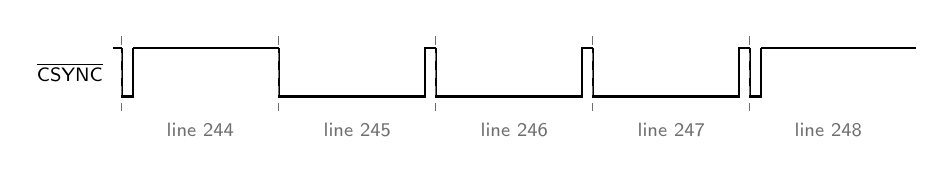
\begin{tikzpicture}[
			x=0.0012\textwidth,
			y=0.62cm,
			lane/.style={font=\scriptsize, anchor=east},
			note/.style={font=\scriptsize, text=sircgray}
		]
		% x is in units of 10 master clocks; five lines of 136.4 units
		\node[lane] at (-8,0.5) {\activelow{CSYNC}};
		\foreach \i in {0,1,2,3,4} {
				\pgfmathsetmacro{\o}{\i*136.4}
				\ifnum\i=0 \draw[thick] (\o,1) -- (\o,0) -- (\o+10,0) -- (\o+10,1);
				\else\ifnum\i=4 \draw[thick] (\o,1) -- (\o,0) -- (\o+10,0) -- (\o+10,1);
					\else
						\draw[thick] (\o,1) -- (\o,0) -- (\o+127.2,0) -- (\o+127.2,1) -- (\o+136.4,1);
					\fi\fi
			}
		\draw[thick] (-8,1) -- (0,1);
		\draw[thick] (10,1) -- (136.4,1);
		\draw[thick] (4*136.4+10,1) -- (682+8,1);
		\foreach \i/\l in {0/244, 1/245, 2/246, 3/247, 4/248} {
				\pgfmathsetmacro{\o}{\i*136.4}
				\draw[dashed, sircgray] (\o,-0.3) -- (\o,1.4);
				\node[note, anchor=north] at (\o+68.2,-0.35) {line \l};
			}
	\end{tikzpicture}
	\caption{Vertical Sync in Lines 245 to 247 (NTSC), with Horizontal Sync before and after}
	\label{fig:signal-vsync}
\end{figure}

\chapter{Programming the Device}
\label{ch:programming}

This chapter collects what a program does in what order. It adds no new rules; each rule is stated where the feature is
described, and the sections of the earlier chapters are cited.

\section{Starting Up}
\label{sec:startup}

At reset the picture is blank (\texttt{GD} is 1), every writable register is zero except \texttt{CONFIG}
(Section~\ref{sec:reset}), and video memory, the palette and the sprite table are undefined. A program starts the
device in this order:

\begin{enumerate}
	\item Install the handler for the vertical sync interrupt, \activelow{NMI}, before anything enables it
	      (Section~\ref{sec:interrupts}).
	\item With the picture still blank, write the palette (\texttt{0x6000}--\texttt{0x60FF}), the tile data and the tilemaps into
	      video memory (Chapter~\ref{ch:memory-map}). Video memory is open to the CPU while \texttt{GD} is 1.
	\item Fill the sprite table, hiding every entry the program does not use by setting its layer field to 3
	      (Section~\ref{sec:sprite-entry}).
	\item Write the tilemap address, tile data address, palette configuration and scroll registers of the backgrounds in use, the
	      \texttt{STILES} register, and the \texttt{TILESIZE} register.
	\item Write \texttt{INTCTL} to enable the interrupts the program uses (\texttt{VIE}, and \texttt{LIE} with \texttt{LINE} for
	      a line-compare interrupt).
	\item Write \texttt{CONFIG} with the mode, the brightness and \texttt{GD} = 0. The picture appears from the next line.
\end{enumerate}

\section{One Frame}
\label{sec:frame-flow}

Figure~\ref{fig:frame-flow} shows a frame as the program sees it. The device draws lines 0 to 223 without help; line 0
is always blank (Section~\ref{sec:first-line}). At the first cycle of line 224 it raises the \activelow{NMI} (if
\texttt{VIE} is set) and sets the \texttt{VBL} bit of the Status register, and the handler has the rest of vertical
blanking, 38 lines or 25,916 cycles on NTSC and 88 lines on PAL, to change video memory, the sprite table and the
registers for the next frame.

\begin{figure}[H]
	\centering
	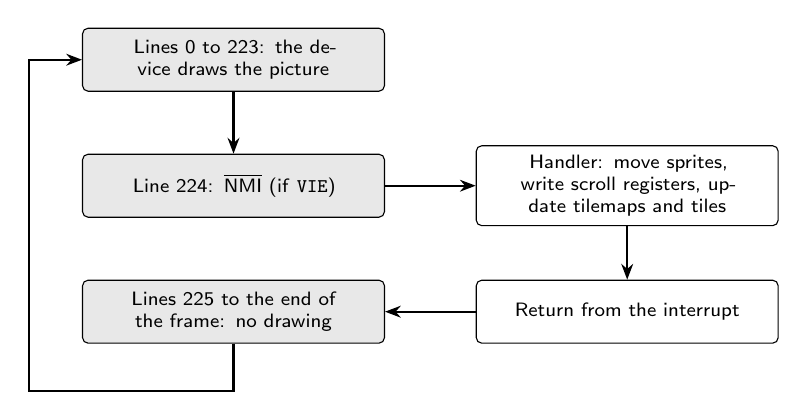
\begin{tikzpicture}[
			box/.style={draw, rounded corners=2pt, minimum height=0.8cm, text width=3.6cm, align=center, font=\scriptsize},
			dev/.style={box, fill=sirclightgray},
			flow/.style={-{Stealth[length=2mm]}, thick}
		]
		\node[dev] (draw) at (0,0) {Lines 0 to 223: the device draws the picture};
		\node[dev] (nmi) at (0,-1.6) {Line 224: \activelow{NMI} (if \texttt{VIE})};
		\node[box] (h1) at (5,-1.6) {Handler: move sprites, write scroll registers, update tilemaps and tiles};
		\node[box] (h2) at (5,-3.2) {Return from the interrupt};
		\node[dev] (blank) at (0,-3.2) {Lines 225 to the end of the frame: no drawing};
		\draw[flow] (draw) -- (nmi);
		\draw[flow] (nmi) -- (h1);
		\draw[flow] (h1) -- (h2);
		\draw[flow] (h2) -- (blank);
		\draw[flow] (blank.south) -- ++(0,-0.6) -| (-2.6,0) -- (draw.west);
	\end{tikzpicture}
	\caption{A Frame}
	\label{fig:frame-flow}
\end{figure}

A program that does not use the interrupt waits for the \texttt{VBL} bit instead: it reads \texttt{STATUS} until bit 7
is set, and it knows how far into the frame it is from \texttt{VLINE}. A program that polls must finish before
\texttt{VBL} falls at line 0, so it reads \texttt{VBL} again before each write that matters near the end.

A \texttt{DMAT} of 255 words takes 522 cycles (Section~\ref{sec:cpu-clock}), so a program doing nothing else could move
at most about 12,600 words in an NTSC vertical blanking interval. A program that needs more than it can move in one
frame spreads the work over several frames, or turns the picture off (\texttt{GD} = 1) for the time it needs.

\section{Programming Cautions}
\label{sec:cautions}

\begin{enumerate}
	\item \textbf{Video memory.} A write to video memory or to the sprite table outside vertical blanking is lost, and a
	      read returns zero, unless \texttt{GD} is 1 (Section~\ref{sec:memory-vram-access}). A program knows video memory is open when \texttt{VBL} in the
	      Status register is set. The palette and the registers can be written at any time.
	\item \textbf{The sprite table.} The table is undefined at reset. A program must hide the entries it does not use before
	      it clears \texttt{GD}, or random sprites appear.
	\item \textbf{NMI.} The \activelow{NMI} cannot be masked. Install the handler before setting \texttt{VIE}. A
	      \texttt{DMAT} that is running at line 224 delays the interrupt until it ends (Section~\ref{sec:interrupts}).
	\item \textbf{Line compare.} The \activelow{IRQ4} line stays asserted until the program writes \texttt{LINE}. A handler
	      that does not write \texttt{LINE}, or clear \texttt{LIE}, is entered again as soon as it returns.
	\item \textbf{Registers during the picture.} The device samples the scroll registers once per line, and a change made during a line takes effect on the next line. It reads the tilemap address, tile data address and palette configuration registers as it fetches, so a change during the visible part of a line can mix old and new settings within that line: change them only in vertical blanking or while \texttt{GD} is 1 (Chapter~\ref{ch:mode2}).
	\item \textbf{Changing mode.} Change \texttt{MODE} only in vertical blanking or while \texttt{GD} is 1. The values 3 to 7
	      of \texttt{MODE} are reserved and must not be written.
	\item \textbf{Reserved registers.} Software must not write the reserved registers and reserved bits
	      (Chapter~\ref{ch:registers}). A read of an open bus offset returns zero.
	\item \textbf{Scroll registers.} The scroll registers are 10 bits. A program keeps its position in a wider variable and
	      writes the low 10 bits; in Mode 2 it also adjusts \texttt{SCRY} when it brings \texttt{SCRX} back past 1024
	      (Section~\ref{sec:m2-moving}).
	\item \textbf{Reading video memory.} A read of video memory takes one wait state, and two straight after a write, and it returns zero outside vertical blanking and forced blank (Section~\ref{sec:signal-vram}). A program keeps in RAM what it will need again, instead of reading it back.
	\item \textbf{Sprites per line.} A line shows at most 32 sprites; the rest are dropped and \texttt{SOV} is set. Read
	      \texttt{SOV} in vertical blanking (Section~\ref{sec:sprite-budget}).
	\item \textbf{Transparent pixels.} Pixel value 0 of a background or a sprite is transparent. If every layer is transparent
	      at a pixel, the device shows palette entry 0 (Section~\ref{sec:compositing}).
	\item \textbf{PAL and NTSC.} A program that depends on the number of lines or the frame rate reads \texttt{OUT} in the
	      Status register.
\end{enumerate}

\chapter{Status and Open Issues}
\label{ch:status}

This chapter lists what the reference simulator implements, where it disagrees with the older design notes on the
project wiki or with itself, and the design questions that remain. It is the list to read before relying on anything
else in the manual.

\section{Implementation Status}

\begin{table}[H]
	\centering
	\begin{tabular}{p{5.8cm}p{3.4cm}p{5.2cm}}
		\toprule
		\textbf{Feature}                                   & \textbf{Status}                                              & \textbf{Notes}                                                                  \\
		\midrule
		Registers, palette and VRAM access                 & Implemented                                                  & Open bus reads zero                                                             \\
		Package, pins, signal timing, video output         & Specified                                                    & The simulator has no pins; Chapters~\ref{ch:package} and~\ref{ch:signal-timing} \\
		Mode 1 backgrounds, 8 by 8 tiles, 32 by 32 maps    & Implemented                                                  & Layer order corrected with the sprite prototype                                 \\
		Mode 1 scrolling (specified)                       & Not yet implemented                                          & Registers stored                                                                \\
		Mode 1 16 by 16 tiles, double tilemaps (specified) & Not yet implemented                                          & Registers stored                                                                \\
		Orthogonal tile flips (specified), priority bit    & Not yet implemented; priority in Mode 3 and the status layer &                                                                                 \\
		2-bit tile data (Mode 1)                           & Not yet implemented                                          &                                                                                 \\
		Graphics disable, brightness (specified)           & Not yet implemented                                          & Bits stored                                                                     \\
		Background disables                                & Modes 2 and 3 only                                           &                                                                                 \\
		Sprites, sprite disables and sizes                 & Prototype                                                    & Proposed, both modes; Chapter~\ref{ch:sprites}                                  \\
		Vertical sync interrupt (NMI)                      & Implemented                                                  & At line 224; on level 4, not the NMI yet                                        \\
		Vertical blanking flag and current line register   & Implemented                                                  & \texttt{VBL} in Status, \texttt{VLINE} at \texttt{0x0018}                       \\
		PAL timing and the output mode flag (specified)    & Not yet implemented                                          &                                                                                 \\
		Blanking-only VRAM access (specified)              & Not yet implemented                                          & Not enforced                                                                    \\
		Forced blank, graphics disable (specified)         & Not yet implemented                                          & GD stored only                                                                  \\
		Mode 2                                             & Prototype                                                    & Proposed; Chapter~\ref{ch:mode2}                                                \\
		Mode 2 status layer (background 3)                 & Prototype                                                    & Proposed; Section~\ref{sec:m2-status-layer}                                     \\
		Mode 2 2-bit isometric tiles                       & Prototype                                                    & Proposed; Section~\ref{sec:m2-two-bit}                                          \\
		Mode 3                                             & Prototype                                                    & Proposed; Chapter~\ref{ch:mode3}                                                \\
		Isometric shading, shadow sprites                  & Prototype                                                    & Proposed; Section~\ref{sec:m2-shading}                                          \\
		2-bit orthogonal tiles                             & Mode 3 and Mode 2 only                                       & Not yet implemented in Mode 1                                                   \\
		\bottomrule
	\end{tabular}
	\caption{Implementation Status}
	\label{tab:status}
\end{table}

\section{Discrepancies}
\label{sec:status-discrepancies}

The following are known differences between this manual's source, the simulator, and its other sources. Each is a
defect to be fixed in the simulator or a decision to be made; the manual describes the intended behavior and notes the
difference.

\begin{enumerate}
	\item \textbf{Register addresses.} The wiki puts the sprite tile data base at offset \texttt{0x0012} and the status at
	      \texttt{0x0013}. The simulator puts the three background palette configuration registers at
	      \texttt{0x0012}--\texttt{0x0014}, the sprite tile data base at \texttt{0x0016} and the status at \texttt{0x0017}.
	      This manual follows the simulator.
	\item \textbf{Palette boundary} (fixed). The simulator used to decode palette offsets \texttt{0x6000}--\texttt{0x6100}
	      inclusive, one past the end of its 256 entries; it now stops at \texttt{0x60FF} (Section~\ref{sec:palette-edge}).
	\item \textbf{Mode 1 layer order} (fixed with the sprite prototype). The simulator used to show background 3 in front of
	      background 1; it now uses the intended order (Section~\ref{sec:m1-priority}).
	\item \textbf{Mode 1 palette sum} (fixed with the sprite prototype). The simulator added the palette offset and the
	      tile value without wrapping, so a large offset could stop the simulator in a debug build; it now wraps, as
	      Mode 2 and Section~\ref{sec:palette-select} do.
	\item \textbf{Status byte order} (fixed). The simulator read the Status register with its bytes swapped relative to every
	      other register; it no longer does.
	\item \textbf{Vertical sync position} (fixed). The interrupt used to be asserted at line 0; it is now asserted at line
	      224, the start of vertical blanking (Chapter~\ref{ch:timing}).
	\item \textbf{Mode 1 picture offset.} The simulator's Mode 1 shows the first 8 pixels of every line blank and draws the
	      tilemap 8 pixels to the right of its position, so the last tile column is never shown. The first two groups of a line
	      are flushed before any data has been fetched (Section~\ref{sec:m1-scrolling}).
	\item \textbf{Clock accounting.} The simulator polls every device once per \texttt{CLKI} cycle, which the video device counts
	      as two master clocks (Section~\ref{sec:cpu-clock}); the terminal device counts one poll as one master clock, so its
	      baud rate is off by a factor of two.
	\item \textbf{VRAM access during rendering.} The specification ignores accesses to video memory and the sprite table outside
	      vertical blanking; the simulator allows them (Chapter~\ref{ch:memory-map}).
\end{enumerate}

\section{Open Design Questions}

\subsection{General}

\begin{itemize}
	\item \textbf{Interrupts.} Specified (Section~\ref{sec:interrupts}): vertical sync on the \activelow{NMI} with no
	      acknowledgement, line compare on \activelow{IRQ4}, held until a write to \texttt{LINE}, both enabled from the Interrupt
	      Control register. The simulator still pulses vertical sync on level 4 and line compare on level 3 for one cycle,
	      with no enable for vertical sync. A one-cycle NMI pulse is one \texttt{CLKI} cycle, which the CPU's edge detector accepts.
	\item \textbf{The wiki.} The project wiki's register map (the sprite tile data base and status register offsets) disagrees with
	      this manual and the simulator, and should be updated from this manual.
	\item \textbf{Version and region.} \texttt{VER} is 1 and the region is fixed when the device is made; the simulator should
	      let both be configured at run time.
	\item \textbf{Package and signals.} The package, the pin assignment and the signal timing of Chapters~\ref{ch:package} and~\ref{ch:signal-timing}
	      are a first sketch, to be confirmed: the 52-pin PLCC; a chip select instead of the segment address bits; \texttt{CLKI} as
	      the only clock; \activelow{BACK}, \activelow{NMI} and \activelow{IRQ4} as open-drain outputs; no access-type or protection
	      inputs; a minimum reset of six cycles; the composite sync widths (a horizontal pulse of 100 master clocks; vertical sync
	      in three lines, 245 to 247, one long pulse in each, no equalising pulses); and the converter and supply pins. The video memory,
	      palette and sprite table are inside the package. Electrical characteristics (levels, delays, frequency range, current,
	      thermal) are not yet specified, as in the \hwmanual{}.
	\item \textbf{DMA.} A DMA transfer into video memory is subject to the same rule as the CPU
	      (Section~\ref{sec:memory-vram-access}), and DMA blocks interrupts, the \activelow{NMI} included, so programs keep
	      transfers short and away from line 224 (Section~\ref{sec:interrupts}).
\end{itemize}

\subsection{Mode 2}

\begin{itemize}
	\item \textbf{Whether to approve it.} Mode 2 narrows the device to one kind of picture. That is its purpose, but it is a
	      decision, not a default.
	\item \textbf{Sprites.} With no free fetch slot, Mode 2 sprites come from a line buffer filled in the blanking
	      interval; the prototype shows that 32 sprites per line of either size fit (Chapter~\ref{ch:sprites}). Whether
	      32 is enough for a vehicle-heavy game, and whether to pay for a second line buffer to double it, is open.
	\item \textbf{The status layer.} Prototyped with a queue of four groups (Section~\ref{sec:m2-status-layer}). Open: whether
	      it should scroll, whether its tiles can be flipped, and whether to use its slots for a third isometric background
	      instead.
	\item \textbf{2-bit tiles.} Prototyped (Sections~\ref{sec:m2-two-bit} and~\ref{sec:flat-two-bit}). Left to the program:
	      the palette size with \texttt{T2}. Open: the Mode 1 implementation.
	\item \textbf{Mode 3.} Prototyped (Chapter~\ref{ch:mode3}). Open: whether the orthogonal backgrounds should have a priority bit to
	      draw in front of sprites, and whether another arrangement of orthogonal and isometric backgrounds is wanted.
	\item \textbf{Shading.} Prototyped (Section~\ref{sec:m2-shading}). Open: whether darkening should have more than one level,
	      and whether a shadow pixel should darken sprites behind it as well as backgrounds.
	\item \textbf{The tilemap entry cache.} Measured and left out (Section~\ref{sec:m2-entry-cache}); worth revisiting if
	      the spare slots are wanted for something else.
	\item \textbf{Rotation of the view.} Ruled out as a register; to show another facing a program needs another set of
	      tiles and map.
	\item \textbf{The symmetric diamond.} The footprint of Table~\ref{tab:m2-footprint} is one pixel narrower at the top than the
	      bottom. A conventionally symmetric diamond does not give a bijection (some texels would be shown twice and
	      some never). The manual keeps the footprint that does. The slicing tool accepts any picture, but diamonds that
	      are to tessellate must be drawn to that footprint.
	\item \textbf{The fixed tilemap size.} A 32 by 32 map is 512 by 512 texels; a transport game would want a larger map and
	      would page it by rewriting the tilemap.
\end{itemize}


\appendix
\chapter{Quick Reference}
\label{app:quick-reference}

\section{Registers}

\begin{table}[H]
	\centering
	\begin{tabular}{llp{7cm}}
		\toprule
		\textbf{Offset}                  & \textbf{Name}                      & \textbf{Fields}                                                                                                                                                        \\
		\midrule
		\texttt{0x0000}                  & \texttt{CONFIG}                    & 15 \texttt{GD}; 14--12 \texttt{B1D}--\texttt{B3D}; 10--8 \texttt{S1D}--\texttt{S3D}; 7 \texttt{SHD}; 6--3 \texttt{BRT}; 2--0 \texttt{MODE} (0, 1, 2 for Modes 1, 2, 3) \\
		\texttt{0x0001}                  & \texttt{TILESIZE}                  & 15--13 \texttt{B1S}--\texttt{B3S}; 11--9 \texttt{S1S}--\texttt{S3S}; 7--5 \texttt{B1X}--\texttt{B3X}; 3--1 \texttt{B1Y}--\texttt{B3Y}                                  \\
		\texttt{0x0002}--\texttt{0x0004} & \texttt{B1MAP}--\texttt{B3MAP}     & Tilemap word address                                                                                                                                                   \\
		\texttt{0x0006}--\texttt{0x0008} & \texttt{B1TILES}--\texttt{B3TILES} & Tile data word address                                                                                                                                                 \\
		\texttt{0x000A}--\texttt{0x000C} & \texttt{B1SCRX}--\texttt{B3SCRX}   & 9--0 scroll amount                                                                                                                                                     \\
		\texttt{0x000E}--\texttt{0x0010} & \texttt{B1SCRY}--\texttt{B3SCRY}   & 9--0 scroll amount                                                                                                                                                     \\
		\texttt{0x0011}                  & \texttt{INTCTL}                    & 1 \texttt{LIE}; 0 \texttt{VIE}                                                                                                                                         \\
		\texttt{0x0012}--\texttt{0x0014} & \texttt{B1PAL}--\texttt{B3PAL}     & 15--8 \texttt{OFFSET}; 2 \texttt{T2}; 1--0 \texttt{SIZE}                                                                                                               \\
		\texttt{0x0015}                  & \texttt{LINE}                      & 8--0 line for the line-compare interrupt; a write acknowledges it                                                                                                      \\
		\texttt{0x0016}                  & \texttt{STILES}                    & Sprite tile data word address                                                                                                                                          \\
		\texttt{0x0017}                  & \texttt{STATUS}                    & 7 \texttt{VBL}; 6 \texttt{LIP}; 5 \texttt{SOV}; 4 \texttt{OUT}; 3--0 \texttt{VER} (read-only)                                                                          \\
		\texttt{0x0018}                  & \texttt{VLINE}                     & 8--0 current line (read-only)                                                                                                                                          \\
		\bottomrule
	\end{tabular}
	\caption{Register Summary}
	\label{tab:app-registers}
\end{table}

\section{Memory Map}

Registers \texttt{0x0000}--\texttt{0x00FF}; palette \texttt{0x6000}--\texttt{0x60FF}; video memory
\texttt{0x8000}--\texttt{0xFFFF} (32,768 words). Everything else is open bus.

\section{Formats}

\begin{description}
	\item[Colour:] bit 15 reserved; bits 14--10 red; bits 9--5 green; bits 4--0 blue.
	\item[Tilemap entry:] bit 15 \texttt{V}; bit 14 \texttt{H}; bit 13 \texttt{P}; bits 12--10 palette selection; bits 9--0 tile
	      number.
	\item[Tile data word:] four 4-bit pixels, leftmost in bits 15--12. Value 0 is transparent.
	\item[Isometric tilemap entry flips:] V darkens, H lightens (both: normal).
	\item[2-bit orthogonal tile:] 8 words, one per row, leftmost pixel in bits 15--14; word at base $+\ 8t + r$.
	\item[Sprite shadow:] value 15 of sprite palette 7 darkens what is behind its layer.
	\item[Palette entry:] $((s \ll k) + \texttt{OFFSET} + v) \bmod 256$, with $k$ = 2, 3, 4, 5 for \texttt{SIZE} 0, 1, 2, 3.
\end{description}

\section{Orthogonal Tiles}

\begin{description}
	\item[16 by 16 tile, 4 bits:] 64 words, quadrants top left, top right, bottom left, bottom right; word at base $+\ 64t + 16q +
		      2(r \bmod 8) + h$.
	\item[Tilemap sizes:] screens of 32 by 32 entries, A B over C D, 1,024 words apart.
	\item[Priority bit:] 1 puts the tile in front of all sprites.
	\item[Reset:] \texttt{CONFIG} = \texttt{0x8078} (blank, full brightness, Mode 1); the other registers are 0.
\end{description}

\section{Mode 1 Addresses}

Tilemap entry: tilemap base $+\ \lfloor x/8 \rfloor + 32\lfloor y/8 \rfloor$.

Tile data word: tile data base $+\ 16t + 2r + h$ for tile $t$, row $r$ and half $h$ of the row.

\section{Mode 2 Formulas}

For the plane pixel $(X, Y) = (x + \texttt{SCRX},\ y + \texttt{SCRY})$:

\begin{align*}
	u   & = Y + \lfloor X/2 \rfloor,      & v   & = Y - \lfloor (X+1)/2 \rfloor,  \\
	c_u & = \lfloor u/16 \rfloor \bmod W, & c_v & = \lfloor v/16 \rfloor \bmod H,
\end{align*}

\noindent with $W$ and $H$ the map's width and height in cells (32 or 64), and the tilemap entry at tilemap base
$+\ 1024 s + 32 (c_v \bmod 32) + (c_u \bmod 32)$, where $s = \lfloor c_v/32 \rfloor (W/32) + \lfloor c_u/32 \rfloor$ is the screen.

For the texel $(t_u, t_v) = (u \bmod 16, v \bmod 16)$ of a tile:

\begin{align*}
	i      & = (t_u - t_v) \bmod 4,                                    \\
	(a, b) & = (t_u - \lfloor i/2 \rfloor,\ t_v + [0, 1, 1, 2]_i),     \\
	w      & = 16 \lfloor ((a - b) \bmod 16)/4 \rfloor + (a \bmod 16),
\end{align*}

\noindent the word $w$ of the tile, at tile data base $+\ 64t + w$, nibble $i$ (0 is bits 15--12).

The top pixel of cell $(c_u, c_v)$ is at the plane pixel $(16(c_u - c_v),\ 8(c_u + c_v))$.


\backmatter

\clearpage
\thispagestyle{empty}
\begin{center}

	\vspace*{1.5cm}

	{\Large\bfseries SIRCADA Reference Manual}

	\vspace{1cm}

	\begin{minipage}{0.8\textwidth}
		This manual describes SIRCADA, the SIRC Analogue Display Adapter: the picture processing unit that turns tiles, tilemaps and palette
		entries in its video memory into a 256 by 224 pixel picture. It is written for the programmers who draw with it,
		the authors of the tools that prepare graphics for it, and the engineers who implement it. What the CPU does when
		it reads and writes the device is the subject of the companion manuals.

		\vspace{0.6cm}

		\textbf{This manual contains:}
		\begin{itemize}
			\item The device's memory map, registers and data formats
			\item Mode 1, three orthogonal tiled backgrounds, and Mode 2, two isometric backgrounds
			\item The scanline timing and the video memory fetch schedule of each mode
			\item The implementation status of every feature and the questions still open
		\end{itemize}
	\end{minipage}

	\vfill

	{\small SILICON INTEGRATED RESEARCH CORPORATION}

\end{center}


\end{document}
